% Options for packages loaded elsewhere
\PassOptionsToPackage{unicode}{hyperref}
\PassOptionsToPackage{hyphens}{url}
%
\documentclass[
  12pt,
  spanish,
]{article}
\usepackage{lmodern}
\usepackage{amssymb,amsmath}
\usepackage{ifxetex,ifluatex}
\ifnum 0\ifxetex 1\fi\ifluatex 1\fi=0 % if pdftex
  \usepackage[T1]{fontenc}
  \usepackage[utf8]{inputenc}
  \usepackage{textcomp} % provide euro and other symbols
\else % if luatex or xetex
  \usepackage{unicode-math}
  \defaultfontfeatures{Scale=MatchLowercase}
  \defaultfontfeatures[\rmfamily]{Ligatures=TeX,Scale=1}
\fi
% Use upquote if available, for straight quotes in verbatim environments
\IfFileExists{upquote.sty}{\usepackage{upquote}}{}
\IfFileExists{microtype.sty}{% use microtype if available
  \usepackage[]{microtype}
  \UseMicrotypeSet[protrusion]{basicmath} % disable protrusion for tt fonts
}{}
\makeatletter
\@ifundefined{KOMAClassName}{% if non-KOMA class
  \IfFileExists{parskip.sty}{%
    \usepackage{parskip}
  }{% else
    \setlength{\parindent}{0pt}
    \setlength{\parskip}{6pt plus 2pt minus 1pt}}
}{% if KOMA class
  \KOMAoptions{parskip=half}}
\makeatother
\usepackage{xcolor}
\IfFileExists{xurl.sty}{\usepackage{xurl}}{} % add URL line breaks if available
\IfFileExists{bookmark.sty}{\usepackage{bookmark}}{\usepackage{hyperref}}
\hypersetup{
  pdflang={es},
  hidelinks,
  pdfcreator={LaTeX via pandoc}}
\urlstyle{same} % disable monospaced font for URLs
\usepackage[margin=2.5cm]{geometry}
\usepackage{longtable,booktabs}
% Correct order of tables after \paragraph or \subparagraph
\usepackage{etoolbox}
\makeatletter
\patchcmd\longtable{\par}{\if@noskipsec\mbox{}\fi\par}{}{}
\makeatother
% Allow footnotes in longtable head/foot
\IfFileExists{footnotehyper.sty}{\usepackage{footnotehyper}}{\usepackage{footnote}}
\makesavenoteenv{longtable}
\usepackage{graphicx}
\makeatletter
\def\maxwidth{\ifdim\Gin@nat@width>\linewidth\linewidth\else\Gin@nat@width\fi}
\def\maxheight{\ifdim\Gin@nat@height>\textheight\textheight\else\Gin@nat@height\fi}
\makeatother
% Scale images if necessary, so that they will not overflow the page
% margins by default, and it is still possible to overwrite the defaults
% using explicit options in \includegraphics[width, height, ...]{}
\setkeys{Gin}{width=\maxwidth,height=\maxheight,keepaspectratio}
% Set default figure placement to htbp
\makeatletter
\def\fps@figure{htbp}
\makeatother
\setlength{\emergencystretch}{3em} % prevent overfull lines
\providecommand{\tightlist}{%
  \setlength{\itemsep}{0pt}\setlength{\parskip}{0pt}}
\setcounter{secnumdepth}{-\maxdimen} % remove section numbering
\ifxetex
  % Load polyglossia as late as possible: uses bidi with RTL langages (e.g. Hebrew, Arabic)
  \usepackage{polyglossia}
  \setmainlanguage[]{spanish}
\else
  \usepackage[shorthands=off,main=spanish]{babel}
\fi

\author{}
\date{}

\begin{document}

\hypertarget{capuxedtulo-7.-anuxe1lisis-e-interpretaciuxf3n-de-resultados}{%
\section{Capítulo 7. Análisis e interpretación de
resultados}\label{capuxedtulo-7.-anuxe1lisis-e-interpretaciuxf3n-de-resultados}}

\hypertarget{marco-metodoluxf3gico}{%
\subsection{7.1 Marco metodológico}\label{marco-metodoluxf3gico}}

\hypertarget{tipo-de-investigaciuxf3n-cualitativa}{%
\subsubsection{7.1.1 Tipo de investigación:
cualitativa}\label{tipo-de-investigaciuxf3n-cualitativa}}

La presente investigación adopta un enfoque cualitativo para
diagnosticar la gestión financiera de Rústico Pizza y Pan, microempresa
del sector restaurantero ubicada en la colonia Ventura Puente de
Morelia, Michoacán. Se eligió este enfoque porque el objetivo del
estudio no es medir frecuencias ni establecer correlaciones
estadísticas, sino comprender en profundidad cómo opera la gestión
financiera dentro de una microempresa específica, identificar las
prácticas informales que la caracterizan y diagnosticar las brechas
entre la situación actual y las prácticas recomendadas por la literatura
especializada.

\textbf{Justificación del enfoque cualitativo frente al cuantitativo.}
Un enfoque cuantitativo resultaría inadecuado para esta investigación
por tres razones fundamentales. En primer lugar, se trata de un estudio
de caso único: la unidad de análisis es una sola microempresa, lo que
impide la construcción de muestras estadísticamente representativas y la
aplicación de técnicas de inferencia. En segundo lugar, los registros
financieros del negocio son informales, heterogéneos e incompletos ---la
libreta de gastos presenta un subregistro del 12.6\%, el registro de
ventas tiene ocho días sin datos y el inventario cubre solo entre 12 y
15 de aproximadamente 50-60 insumos---, lo que significa que los datos
disponibles no cumplen los requisitos de estandarización y completitud
que exigen los métodos estadísticos. En tercer lugar, los fenómenos que
se busca comprender ---las prácticas de registro, las lógicas de
decisión del propietario, las dinámicas informales de gestión--- son de
naturaleza interpretativa y contextual, no reducibles a variables
numéricas sin perder su significado.

\textbf{Pertinencia del estudio de caso único.} El diseño de la
investigación es de tipo descriptivo y exploratorio, orientado al
estudio de caso único. Yin (2018) argumenta que el estudio de caso único
se justifica cuando se presenta un caso revelador, es decir, cuando el
investigador tiene la oportunidad de observar y analizar un fenómeno que
previamente era inaccesible para la investigación científica. Rústico
Pizza y Pan reúne esta característica: las prácticas financieras
internas de una microempresa familiar del sector restaurantero rara vez
son accesibles para un análisis externo, porque operan en un ámbito
privado donde los registros son personales y las decisiones se toman
informalmente. La apertura de los propietarios para compartir
documentos, acceso a cuentas bancarias y testimonios detallados
constituye una oportunidad de observación que justifica el diseño de
caso único.

\textbf{Pertinencia para microempresas.} El enfoque cualitativo resulta
particularmente pertinente para el estudio de microempresas porque, como
señala la literatura, este tipo de organizaciones opera con dinámicas
que no siempre son capturables mediante instrumentos estandarizados: los
registros son informales, las decisiones se basan en la experiencia del
propietario y las prácticas financieras están profundamente ligadas al
contexto familiar y operativo del negocio. En este sentido,
García-Moreno et al.~(2019) argumentan que ``la investigación documental
permite analizar los resultados de estudios empíricos y fuentes
secundarias para identificar los factores que determinan el nivel de
gestión financiera en las PyMES, lo que facilita un diagnóstico
situacional financiero que promueva la competitividad
empresarial''.\footnote{García-Moreno, S. M., Montoya-del-Corte, J. y
  Fernández-Laviada, A. (2019). Financial management practices in small
  enterprises: an empirical study. \emph{International Journal of
  Entrepreneurial Behaviour and Research}, 25(8), 1751-1776.
  https://doi.org/10.1108/IJEBR-11-2018-0726} La informalidad de los
registros hace que los datos no sean capturables con instrumentos
estandarizados: una libreta con manchas de café y páginas desprendidas,
notas de proveedor acumuladas en una bolsa de plástico y cantidades de
inventario anotadas con signos de interrogación (``Champiñones --- 0.8
kg (?)'') son fuentes de información que requieren interpretación
cualitativa, no codificación estadística.

\textbf{Periodo de análisis.} El periodo de análisis comprende los meses
de diciembre de 2025 a febrero de 2026, lapso que permite observar tanto
la operación regular como los picos estacionales. Este periodo es
representativo porque incluye temporada alta (diciembre, con eventos
navideños y mayor afluencia familiar) y temporada de ajuste (enero,
típicamente el mes más bajo en ventas para el sector restaurantero), lo
que permite capturar la variabilidad estacional del negocio y evitar
conclusiones sesgadas por un periodo atípico. Los promedios diarios de
ventas registrados confirman esta variabilidad: \$3,467 en diciembre,
\$3,892 en enero y \$4,115 en febrero.

\hypertarget{tuxe9cnicas-e-instrumentos-de-recolecciuxf3n}{%
\subsubsection{7.1.2 Técnicas e instrumentos de
recolección}\label{tuxe9cnicas-e-instrumentos-de-recolecciuxf3n}}

Para la recolección de datos se emplearon tres técnicas complementarias
que, en conjunto, permiten triangular la información y fortalecer la
credibilidad de los hallazgos: la entrevista semiestructurada, la
observación directa y el análisis documental.

\textbf{Entrevista semiestructurada.} Se realizó una entrevista
semiestructurada al fundador y operador principal del negocio, Martín
Valadés Cendejas, el 18 de febrero de 2026 en el local de Rústico Pizza
y Pan, con una duración aproximada de 45 minutos. La guía de entrevista
se organizó en siete bloques temáticos que cubren las dimensiones clave
de la gestión financiera de una microempresa:

\begin{enumerate}
\def\labelenumi{\arabic{enumi}.}
\tightlist
\item
  Datos generales y contexto del negocio (historia, equipo, productos,
  perfil del cliente).
\item
  Registro y control de ingresos (proceso de registro de ventas, métodos
  de pago, facturación, ventas mensuales).
\item
  Registro y control de gastos (quién registra, qué rubros, gastos
  principales, separación personal/negocio).
\item
  Gestión de costos e inventario (costeo por producto, control de
  inventario, fijación de precios).
\item
  Flujo de caja y tesorería (disponibilidad de efectivo, pagos a
  proveedores, fondo de emergencia).
\item
  Reportes, análisis y toma de decisiones (estados financieros,
  criterios de decisión, áreas de incertidumbre).
\item
  Expectativas y necesidades tecnológicas (funcionalidades deseadas,
  disposición a adoptar herramientas).
\end{enumerate}

El formato semiestructurado permitió seguir la guía temática mientras se
profundizaba en las respuestas del entrevistado, obteniendo información
rica y contextualizada que un cuestionario cerrado no habría capturado.
Las respuestas se transcribieron íntegramente y se codificaron por
categorías temáticas para su análisis posterior.

\textbf{Observación directa.} De manera simultánea a la entrevista, se
realizó una sesión de observación directa en el local durante tres horas
(11:00 a 14:00 del 18 de febrero de 2026), que incluyó parte del horario
de máxima actividad. El propósito fue complementar la información
declarada en la entrevista con evidencia observacional de primera mano.
Se registraron las siguientes dimensiones:

\begin{itemize}
\tightlist
\item
  Condiciones del local y áreas de trabajo (espacio de atención al
  público, cocina, zona administrativa).
\item
  Ubicación y estado de conservación de los documentos financieros
  físicos.
\item
  Dinámica operativa: proceso de atención al cliente, registro de
  ventas, manejo de efectivo.
\item
  Infraestructura tecnológica disponible.
\item
  Interacción y coordinación del equipo de trabajo.
\end{itemize}

Las notas de observación se registraron en una guía estructurada
organizada por secciones temáticas, lo que facilitó el cruce posterior
con la información de la entrevista y el análisis documental.

\textbf{Análisis documental.} Se realizó una revisión sistemática de
diez documentos financieros y operativos que el negocio genera, mantiene
o conserva. Los documentos se recopilaron en dos etapas: una primera
etapa durante la visita presencial del 18 de febrero de 2026 (acceso
directo a libretas, carpetas, archivos de Excel y aplicación bancaria),
y una segunda etapa mediante la recepción de documentos complementarios
compartidos vía WhatsApp entre el 19 y el 28 de febrero de 2026 por
Mariana Torres Guzmán, cofundadora del negocio.

Cada documento fue examinado mediante fichas de análisis estandarizadas
que evalúan cinco criterios: existencia, periodicidad de actualización,
completitud de los registros, confiabilidad de los datos y formato de
conservación. Los diez documentos analizados fueron:

\begin{longtable}[]{@{}clll@{}}
\toprule
\# & Documento & Formato & Periodicidad\tabularnewline
\midrule
\endhead
1 & Registro de ventas diarias & Excel & Diario (con
omisiones)\tabularnewline
2 & Libreta de gastos & Cuaderno físico & Semanal\tabularnewline
3 & Corte de caja diario & Hoja manuscrita & Diario (con
omisiones)\tabularnewline
4 & Notas de proveedores & Notas de papelería & Por
compra\tabularnewline
5 & Estado de cuenta bancario & App bancaria & Mensual\tabularnewline
6 & Inventario informal & Hoja suelta manuscrita & Quincenal
(irregular)\tabularnewline
7 & Tabla de costos por producto & Excel & Estática (marzo
2025)\tabularnewline
8 & Flujo de caja mensual & Construido por el investigador &
Mensual\tabularnewline
9 & Recibos de nómina informal & Hoja manuscrita &
Quincenal\tabularnewline
10 & Registro de ventas por producto & Libreta de Sofía & Diario
(parcial)\tabularnewline
\bottomrule
\end{longtable}

La triangulación de las tres fuentes ---entrevista, observación y
documentos--- permitió validar hallazgos, identificar inconsistencias
entre lo declarado y lo documentado, y construir un diagnóstico integral
que no depende de una sola fuente de información. Como sostiene Zamora
Aray y Loor Alcívar (2025), ``los administradores y contadores de las
unidades estudiadas constituyen los informantes claves; asimismo, la
guía de observación permite verificar in situ las prácticas de control
interno y gestión financiera declaradas''.\footnote{Zamora Aray, E. A. y
  Loor Alcívar, M. I. (2025). Control interno y gestión financiera de
  las PyMEs de servicios del Cantón Manta. \emph{Horizon Nexus Journal},
  3(2). https://doi.org/10.70881/hnj/v3/n2/67}

\begin{center}\rule{0.5\linewidth}{0.5pt}\end{center}

\hypertarget{situaciuxf3n-actual-de-la-informaciuxf3n-financiera}{%
\subsection{7.2 Situación actual de la información
financiera}\label{situaciuxf3n-actual-de-la-informaciuxf3n-financiera}}

Esta sección organiza los hallazgos del diagnóstico en torno a tres ejes
que corresponden directamente a la primera pregunta de investigación:
\emph{¿en qué medida la información financiera de Rústico Pizza y Pan se
encuentra integrada, estructurada y estandarizada?} Los tres ejes
---integración, estructura y estandarización--- permiten demostrar que
las deficiencias identificadas no son accidentales ni menores, sino que
reflejan la ausencia de un sistema formal de gestión financiera.

\hypertarget{integraciuxf3n-de-la-informaciuxf3n-financiera}{%
\subsubsection{7.2.1 Integración de la información
financiera}\label{integraciuxf3n-de-la-informaciuxf3n-financiera}}

La integración se refiere a la capacidad de conectar las distintas
fuentes de información financiera para obtener una visión consolidada
del negocio. En Rústico Pizza y Pan, los diez documentos financieros
identificados existen como silos aislados que nunca se cruzan entre sí
de manera sistemática.

\textbf{Silos documentales.} El registro de ventas (Excel) no se vincula
con la tabla de costos por producto, lo que impide calcular
automáticamente el costo de ventas diario. Las notas de proveedores (47
notas en papel acumuladas en una bolsa de plástico) no se concilian con
la libreta de gastos: al cruzar ambas fuentes, se encontraron 9 compras
documentadas en notas de remisión por un total de \$7,430 que no
aparecen en la libreta, lo que representa un subregistro del 12.6\% del
gasto en proveedores. El estado de cuenta bancario, por su parte,
muestra una discrepancia de \$2,370 entre las ventas con tarjeta
reportadas en los cortes de caja (\$101,600) y los depósitos netos
ajustados por comisión (\$99,230), una diferencia que nunca ha sido
investigada por el negocio.

\textbf{Circuito paralelo de efectivo.} Se estima que entre el 40\% y el
50\% de los ingresos en efectivo nunca transitan por la cuenta bancaria,
sino que se destinan directamente a compras en efectivo, pagos de nómina
y retiros personales del propietario. Este circuito paralelo genera un
flujo de información invisible: las transacciones ocurren pero no se
documentan ni se integran con los demás registros. El patrón de
depósitos en efectivo a sucursal (entre \$5,000 y \$12,000, con
frecuencia irregular de una a tres veces por mes) confirma que solo una
fracción del efectivo recaudado llega a la cuenta bancaria.

\textbf{Tabla de costos desconectada.} La tabla de costos por producto,
elaborada en marzo de 2025, nunca ha sido cruzada con el registro de
ventas. En consecuencia, es imposible calcular de manera automática
indicadores tan básicos como el costo de ventas diario, el margen bruto
por producto o la rentabilidad comparada entre las distintas líneas del
menú. Esta desconexión constituye una de las brechas más críticas del
diagnóstico, porque impide al negocio identificar cuáles productos son
los más y los menos rentables.

\hypertarget{estructura-de-los-registros-financieros}{%
\subsubsection{7.2.2 Estructura de los registros
financieros}\label{estructura-de-los-registros-financieros}}

La estructura se refiere a la homogeneidad de los formatos de registro y
a la existencia de catálogos y clasificaciones que permitan la
agregación y el análisis de los datos.

\textbf{Heterogeneidad de formatos.} Los diez documentos financieros del
negocio se mantienen en al menos cinco formatos distintos: archivos de
Excel (registro de ventas, tabla de costos), cuaderno físico (libreta de
gastos), hojas sueltas manuscritas (inventario, cortes de caja, recibos
de nómina), notas de papelería preimpresas (proveedores) y aplicación
bancaria digital (estado de cuenta). Esta heterogeneidad impide la
consolidación automática de la información y obliga a un proceso manual
de transcripción, clasificación y cruce que en la práctica nunca se
realiza.

\textbf{Ausencia de catálogos.} No existe un catálogo de cuentas de
gastos ni una nomenclatura estandarizada para los insumos. Un mismo tipo
de gasto aparece registrado como ``Queso'', ``Cremería Don Pancho'' y
``Lácteos proveedor'' en distintas entradas de la libreta, lo que
dificulta la agregación por categoría. De los aproximadamente 50-60
insumos que maneja el negocio, solo entre 12 y 15 se inventarían
periódicamente, y las cantidades registradas son aproximaciones
visuales, no mediciones exactas: un registro señala ``Queso Oaxaca ---
3.5 kg (aprox.)'' y otro ``Champiñones --- 0.8 kg (?)'', donde el signo
de interrogación delata la incertidumbre del propio registrador.

\textbf{Costeo desactualizado.} La única tabla de costos por producto
fue elaborada en marzo de 2025 y no ha sido actualizada en ocho meses.
Los precios de los insumos clave han aumentado significativamente desde
entonces: el queso Oaxaca pasó de \$105/kg a \$130/kg (+23.8\%) y la
harina de \$220 a \$275 por bulto de 44 kg (+25\%). El negocio opera con
la percepción de que sus márgenes son adecuados, cuando en realidad se
han erosionado sin que los propietarios lo adviertan. Dos productos
incorporados al menú después de marzo ---la pizza de huitlacoche con
elote y la pizza de chorizo con papa--- nunca han sido costeados. Martín
expresó en la entrevista: ``lo que no calculamos bien son los costos
indirectos: el gas, la luz, el tiempo, el desgaste del horno. O sea,
sabemos que ganamos, pero el margen exacto producto por producto, no lo
tenemos.''

\hypertarget{estandarizaciuxf3n-de-los-procesos-financieros}{%
\subsubsection{7.2.3 Estandarización de los procesos
financieros}\label{estandarizaciuxf3n-de-los-procesos-financieros}}

La estandarización se refiere a la existencia de procedimientos formales
y consistentes para el registro, la clasificación y el análisis de la
información financiera. En Rústico, la ausencia de procedimientos
estandarizados genera vulnerabilidades en la calidad de los datos.

\textbf{Registro de ventas dependiente de la memoria.} La observación
directa confirmó que durante periodos de alta demanda (entre 13:00 y
13:45 horas), Sofía Valadés prioriza la atención y el cobro sobre el
registro: se observó que atendió tres clientes consecutivos sin anotar
en la libreta y después intentó reconstruir las ventas de memoria. En
una de ellas dudó del monto exacto. No se emite ticket ni comprobante
impreso al cliente. En el periodo analizado se identificaron ocho días
sin registro de ventas en el archivo digital, y el desglose por producto
solo está disponible para aproximadamente el 65\% de los días.

\textbf{Mezcla de finanzas personales y del negocio.} La cuenta bancaria
a nombre de Martín funciona simultáneamente como cuenta del negocio y
cuenta personal. Se identificaron \$11,747 en gastos personales
realizados desde esta cuenta en el trimestre (6.7\% de los egresos
totales): compras en supermercado, cargas de gasolina, un pago a Amazon
y una suscripción a plataforma de streaming, entre otros. El fenómeno es
bidireccional: también se documentaron casos en que Martín paga gastos
del negocio con su tarjeta personal. Martín reconoció: ``siempre decimos
`hay que separar todo bien', pero no lo hemos logrado al cien por
ciento.''

\textbf{Toma de decisiones sin base documental.} El negocio no genera
ningún tipo de reporte financiero formal: ni estado de resultados, ni
balance general, ni flujo de caja. Martín confirmó en la entrevista que
las decisiones se toman ``mucho en el instinto y en la experiencia'', y
que cuando decidieron subir precios ``fue porque veíamos que los costos
ya nos estaban comiendo y que la competencia también estaba subiendo'',
sin realizar un análisis formal de costos ni márgenes.

\textbf{El ciclo de opacidad financiera.} Las deficiencias en
integración, estructura y estandarización descritas en esta sección no
son problemas aislados sino que se retroalimentan, formando un ciclo de
opacidad financiera que se representa en la siguiente figura:

\begin{figure}
\centering
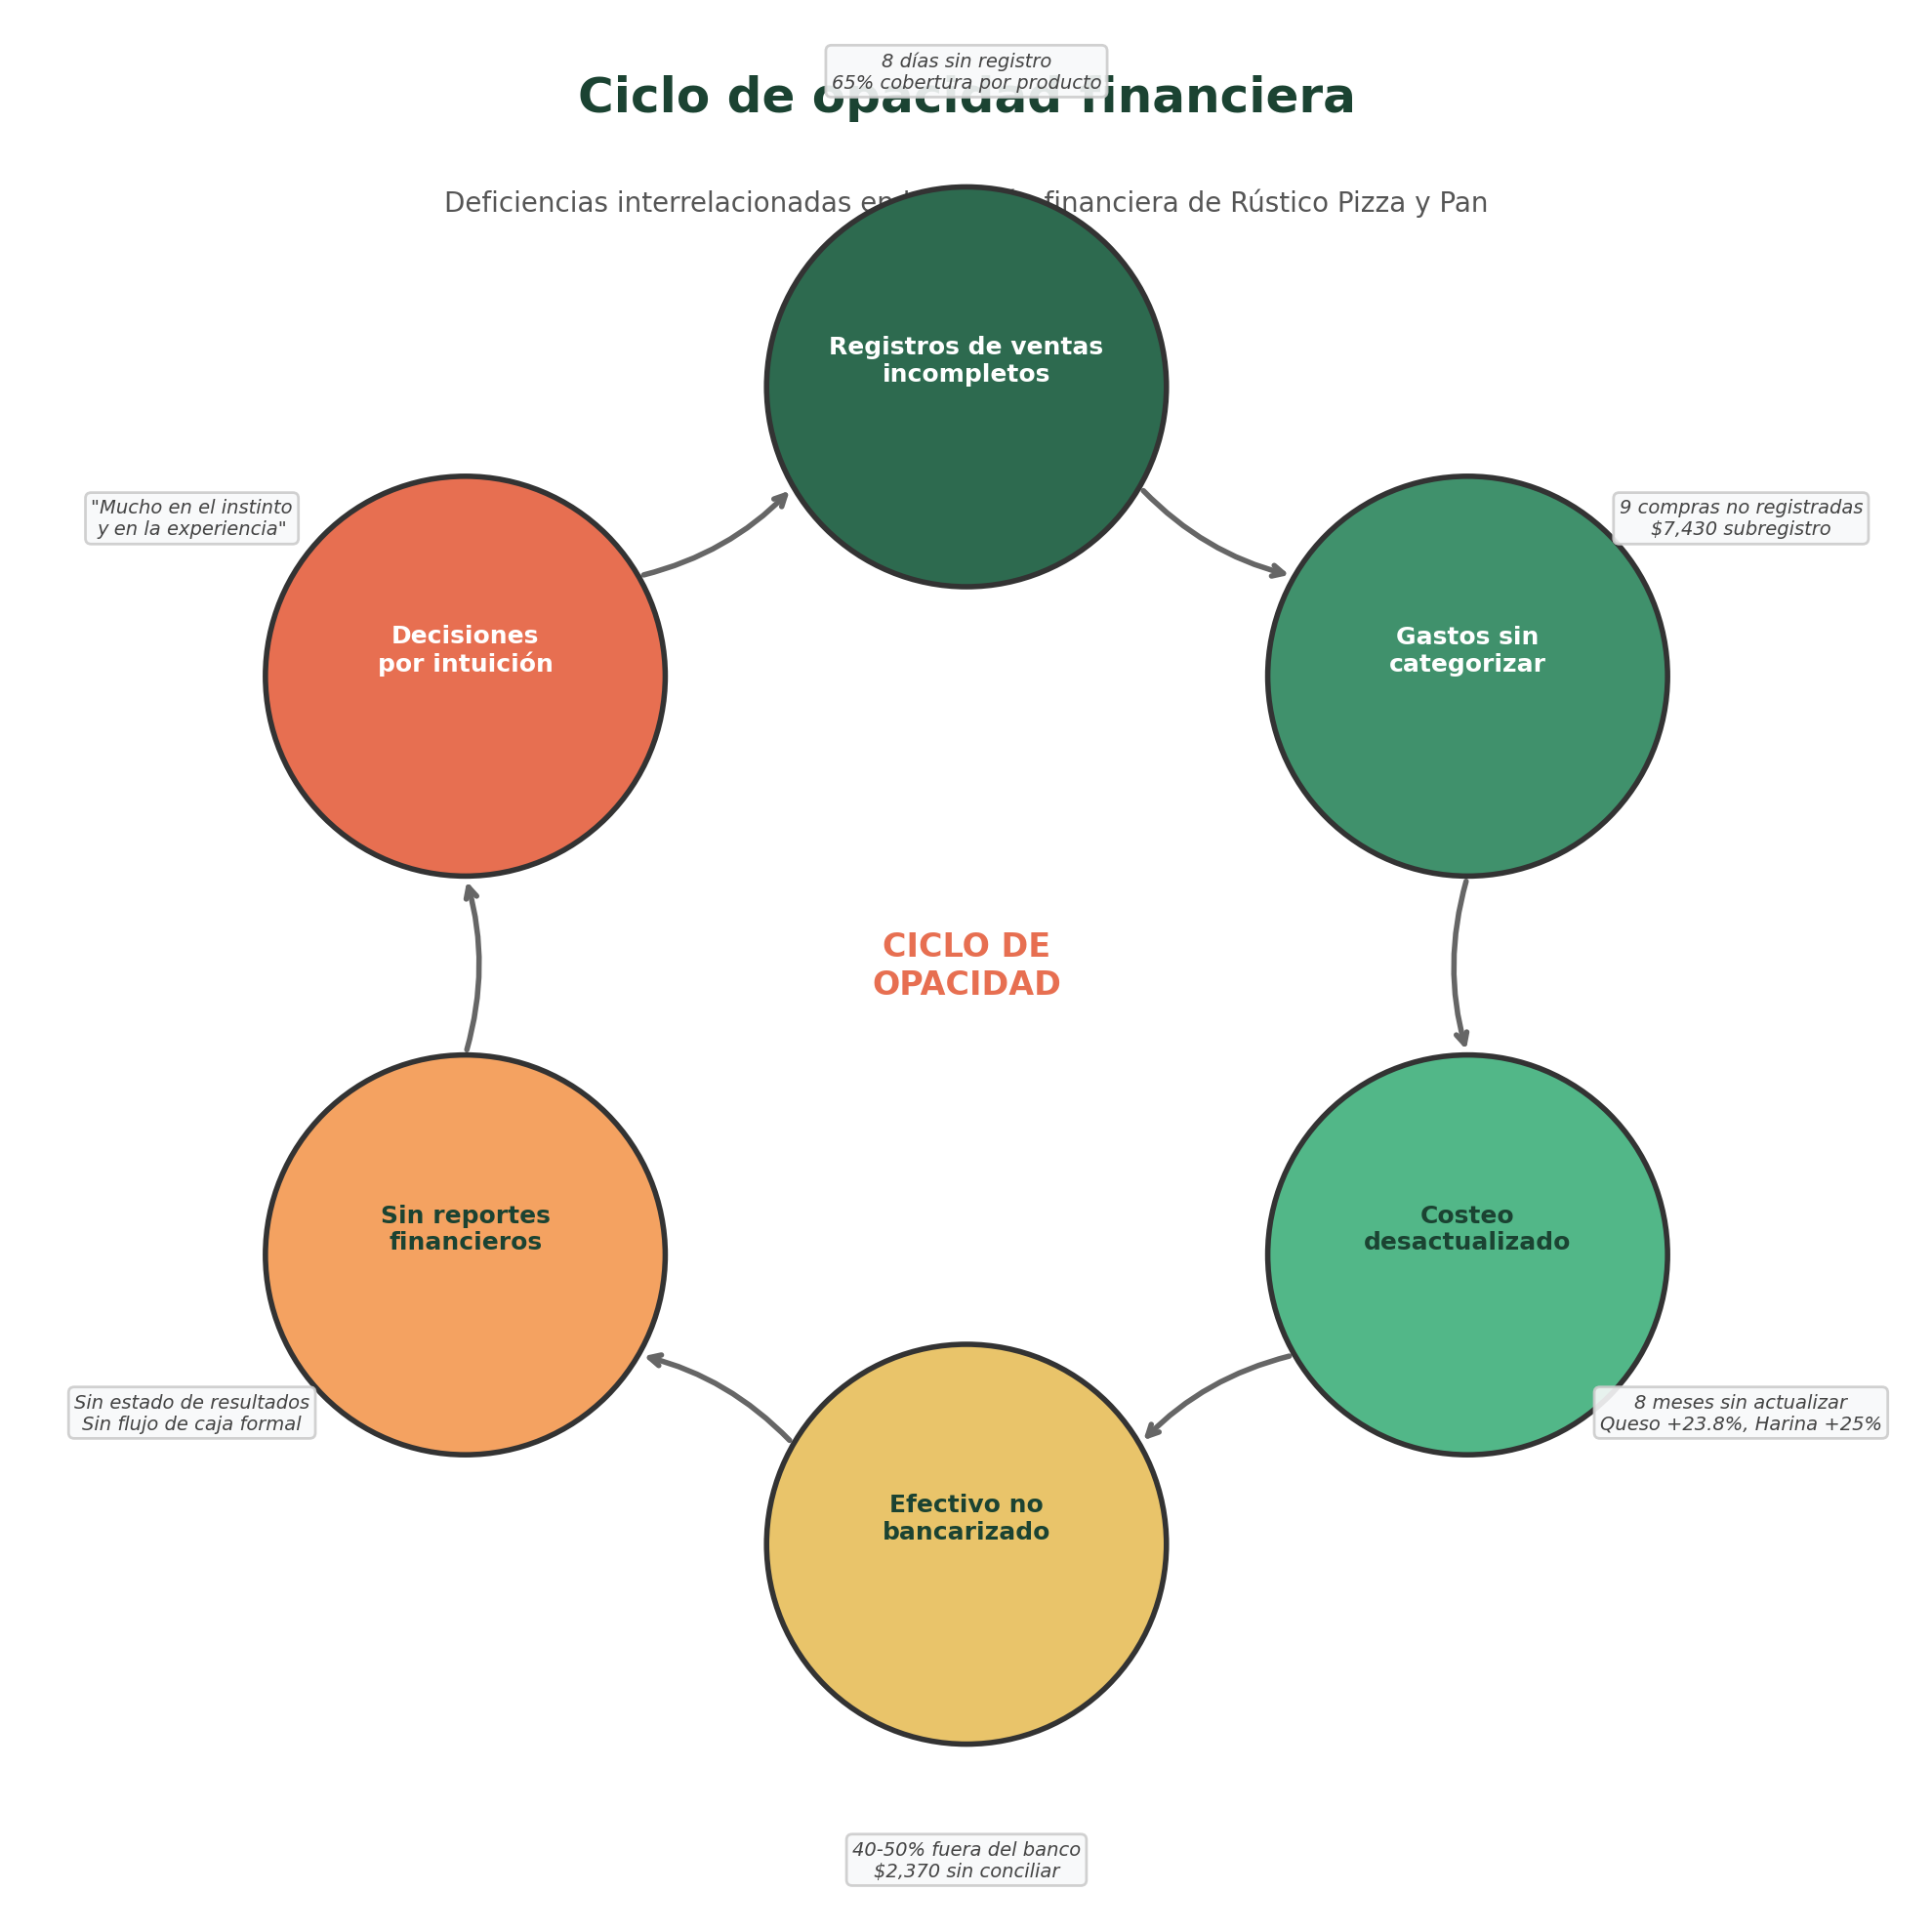
\includegraphics{diagramas/fig4_ciclo_opacidad.png}
\caption{Ciclo de opacidad financiera de Rústico Pizza y Pan}
\end{figure}

\emph{Figura 4. Ciclo de opacidad financiera. Las seis deficiencias
principales se refuerzan mutuamente: los registros incompletos impiden
categorizar gastos, lo cual impide actualizar costos, lo cual se
compensa con efectivo no bancarizado, lo cual imposibilita generar
reportes, lo cual obliga a decidir por intuición, lo cual perpetúa los
registros incompletos.}

La síntesis de estos hallazgos confirma que la gestión financiera de
Rústico Pizza y Pan presenta las características típicas de las
microempresas mexicanas documentadas en la literatura: informalidad en
los registros, mezcla de finanzas personales y empresariales, ausencia
de costeo formal y toma de decisiones basada en la percepción del
propietario. Lo relevante del diagnóstico es que la información
financiera del negocio \textbf{no se encuentra integrada, estructurada
ni estandarizada}, y que esta situación es consecuencia directa de la
\textbf{ausencia de un sistema formal de gestión}. Los datos existen
---hay una libreta, un Excel, notas de proveedor, una cuenta
bancaria---, pero están dispersos en formatos incompatibles, no se
cruzan entre sí y no se transforman en información útil para la toma de
decisiones.

\begin{center}\rule{0.5\linewidth}{0.5pt}\end{center}

\hypertarget{interpretaciuxf3n-de-resultados}{%
\subsection{7.3 Interpretación de
resultados}\label{interpretaciuxf3n-de-resultados}}

\hypertarget{relaciones-entre-las-deficiencias-diagnosticadas}{%
\subsubsection{7.3.1 Relaciones entre las deficiencias
diagnosticadas}\label{relaciones-entre-las-deficiencias-diagnosticadas}}

Los hallazgos descritos en la sección anterior revelan un patrón
consistente: las deficiencias en la gestión financiera de Rústico Pizza
y Pan no son problemas aislados, sino que están interrelacionados y se
refuerzan mutuamente. A continuación se analizan las cinco relaciones
más significativas.

\textbf{Relación entre registros incompletos y capacidad de decisión.}
La ausencia de un registro de ventas completo y sistematizado (8 días
sin datos, sin desglose por producto en el 35\% de los días) priva al
propietario de la información básica para conocer la demanda real por
producto, identificar tendencias estacionales y calcular indicadores
como el ticket promedio. Los datos reconstruidos a partir de la libreta
de Sofía indican que las pizzas representan el 62\% de los ingresos, la
panadería el 24\% y las bebidas el 11\%, con un ticket promedio de \$287
por transacción (\$342 en fines de semana y \$245 entre semana). Sin
embargo, esta información solo está disponible para aproximadamente el
65\% de los días del periodo, y el propio negocio desconoce estos datos
porque nunca se han analizado de manera sistemática. Bravo et al.~(2018)
encontraron que ``los sistemas de información incrementan la efectividad
en la operación de procesos y permiten un control más efectivo de las
actividades organizacionales, siendo asociados con una reducción del
10\% en los costos operativos''.\footnote{Bravo, F., Rubio, J. y
  Calderón, L. (2018). The role of financial information in small
  enterprise management. \emph{Journal of Business Research}, 93,
  422-432. https://doi.org/10.1016/j.jbusres.2017.12.006}

\textbf{Relación entre la informalidad del registro de gastos y la
distorsión del resultado financiero.} El subregistro del 12.6\% de
gastos detectado al cruzar la libreta con las notas de proveedores
implica que el negocio subestima sus egresos reales en aproximadamente
\$7,430 trimestrales (\$2,477 mensuales). A esto se suma la mezcla de
\$3,840 en gastos personales dentro de los registros del negocio, lo que
distorsiona en sentido contrario: los egresos operativos aparentan ser
mayores de lo que realmente son. El efecto neto es que el negocio no
conoce con precisión ni cuánto gasta ni en qué lo gasta. Según los datos
del flujo de caja reconstruido por el investigador, el flujo neto del
trimestre fue positivo (\$24,545 en diciembre, \$36,145 en enero y
\$29,415 en febrero), pero estas cifras contienen un margen de error
significativo derivado de las deficiencias documentales.

\textbf{Relación entre la desactualización del costeo y la erosión de
márgenes.} La tabla de costos de marzo de 2025 calcula un costo de
materia prima de \$42 para la pizza Margarita (vendida a \$120), lo que
implicaría un margen bruto del 65\%. Sin embargo, con el incremento
documentado del queso Oaxaca (+23.8\%) y la harina (+25\%), el costo
real actual es superior. El negocio opera con la percepción de que sus
márgenes son adecuados, cuando en realidad se han erosionado sin que los
propietarios lo adviertan. Al no existir un vínculo entre la tabla de
costos y el registro de ventas, es imposible calcular automáticamente el
costo de ventas diario ni identificar cuáles productos son los más y los
menos rentables.

\textbf{Relación entre el circuito de efectivo no bancarizado y la
imposibilidad de conciliación.} La existencia de un flujo paralelo de
efectivo (40-50\% de los ingresos que nunca transitan por el banco) hace
que el estado de cuenta bancario sea una representación parcial e
incompleta de la realidad financiera del negocio. La discrepancia
acumulada de \$2,370 entre las ventas con tarjeta reportadas en cortes
de caja y los depósitos netos ajustados por comisión ilustra las
dificultades de conciliación incluso en la porción bancarizada. Esta
opacidad financiera impide que el negocio tenga una visión consolidada
de su posición de efectivo real, lo que explica episodios de tensión
financiera como los reportados por Martín: ``A principio de mes, cuando
toca pagar renta, sueldos, proveedores, y todavía no hemos juntado
suficiente de las ventas de los primeros días. Esos días sí se siente la
presión.''

\textbf{Relación entre la ausencia de reportes y la toma de decisiones
intuitiva.} La culminación de todas las deficiencias anteriores es la
inexistencia de reportes financieros que permitan una toma de decisiones
informada. Martín reconoció que las decisiones de precio, contratación e
inversión se basan en ``el instinto y la experiencia'' y no en evidencia
cuantitativa. Esto genera un riesgo latente: mientras el negocio opere
en condiciones estables, la intuición puede ser suficiente, pero ante
cambios significativos del entorno (inflación sostenida en insumos,
entrada de competidores, cambios regulatorios), la ausencia de
información financiera precisa limita la capacidad de respuesta y
adaptación.

\hypertarget{la-necesidad-de-un-sistema-hallazgo-del-diagnuxf3stico}{%
\subsubsection{7.3.2 La necesidad de un sistema: hallazgo del
diagnóstico}\label{la-necesidad-de-un-sistema-hallazgo-del-diagnuxf3stico}}

Las cinco relaciones descritas en la sección anterior conducen a una
conclusión que no fue una premisa de la investigación, sino un hallazgo
que emerge del propio diagnóstico: las deficiencias identificadas en la
gestión financiera de Rústico Pizza y Pan no son problemas puntuales que
puedan resolverse de manera aislada. Son manifestaciones de un problema
sistémico ---la ausencia de un mecanismo que integre, estructure y
estandarice la información financiera--- y, por lo tanto, requieren una
solución sistémica.

\textbf{Las soluciones puntuales son insuficientes.} Arreglar un solo
documento ---por ejemplo, digitalizar la libreta de gastos--- no
resuelve el problema de fondo. Si se digitaliza la libreta pero no se
conecta con el registro de ventas, la tabla de costos y el estado de
cuenta bancario, se sigue operando con silos de información que no se
cruzan. Si se actualiza la tabla de costos pero no se vincula con las
ventas diarias, el costeo vuelve a quedar obsoleto en cuestión de
semanas. Si se separan las cuentas bancarias pero no se implementa un
catálogo de cuentas para los gastos, la categorización seguirá siendo
inconsistente. El diagnóstico muestra que las deficiencias están
interconectadas y que abordarlas de manera fragmentada perpetuaría el
ciclo de opacidad.

\textbf{El patrón sistémico señala la necesidad de un sistema
integrador.} Lo que el diagnóstico revela es que Rústico ya genera los
datos: hay un registro de ventas, hay una libreta de gastos, hay notas
de proveedor, hay cortes de caja, hay un estado de cuenta bancario. El
problema no es la ausencia total de información, sino su
\textbf{fragmentación}, su \textbf{falta de integración} y su
\textbf{desactualización}. La conclusión que emerge naturalmente del
análisis es que se necesita un mecanismo ---un sistema--- que tome esos
datos dispersos, los conecte entre sí y los transforme en información
útil para la toma de decisiones.

\textbf{La pregunta que surge del diagnóstico.} Si la necesidad de un
sistema es un hallazgo del diagnóstico, la pregunta que sigue es: ¿qué
tipo de sistema? ¿Un software comercial genérico? ¿Un ERP empresarial?
¿Una solución diseñada a la medida de las necesidades identificadas?
Esta pregunta se aborda en la siguiente sección, donde se evalúan las
alternativas disponibles y se presenta el diseño conceptual del sistema
que responde directamente a las deficiencias documentadas.

\begin{center}\rule{0.5\linewidth}{0.5pt}\end{center}

\hypertarget{impacto-de-los-resultados}{%
\subsection{7.4 Impacto de los
resultados}\label{impacto-de-los-resultados}}

Esta sección responde a la segunda pregunta de investigación:
\emph{¿cómo podría un sistema modular de gestión financiera organizar la
información y facilitar su análisis para apoyar la toma de decisiones?}
A partir de la necesidad identificada en la sección anterior, se
presenta la justificación, el diseño conceptual y el impacto esperado
del sistema propuesto.

\hypertarget{justificaciuxf3n-sistema-modular-a-la-medida-vs.-alternativas}{%
\subsubsection{7.4.1 Justificación: sistema modular a la medida
vs.~alternativas}\label{justificaciuxf3n-sistema-modular-a-la-medida-vs.-alternativas}}

Antes de presentar el diseño del sistema, es necesario justificar por
qué se propone una solución modular diseñada a la medida del
diagnóstico, en lugar de adoptar una herramienta comercial existente. Se
evaluaron tres alternativas.

\textbf{¿Por qué no un ERP completo como Odoo?} Los sistemas de
planificación de recursos empresariales (ERP) como Odoo ofrecen una
solución integral con más de 30 módulos (contabilidad, CRM, inventario,
recursos humanos, comercio electrónico, entre otros). Sin embargo, para
una microempresa de 4 empleados como Rústico, un ERP presenta
desventajas significativas. El costo de implementación oscila entre
\$15,000 y \$80,000 MXN cuando se incluye la contratación de un
consultor para la configuración inicial, migración de datos y
capacitación. Requiere infraestructura de servidor (local o en la nube)
y soporte técnico continuo. La curva de aprendizaje es alta:
García-Moreno et al.~(2019) señalan que las PyMEs frecuentemente
abandonan los sistemas de gestión cuando su complejidad supera la
capacidad operativa del personal disponible. Govea Souza (2021)
documenta que la implementación de un ERP puede tardar entre 3 y 6 meses
con acompañamiento profesional, un horizonte temporal que excede las
necesidades inmediatas del negocio. En síntesis, un ERP es una solución
sobredimensionada para una microempresa que aún no tiene un catálogo de
cuentas.

\textbf{¿Por qué no un POS comercial genérico?} Los sistemas de punto de
venta comerciales (Square, Poster POS, iFood) resuelven parcialmente el
problema de registro de ventas (H1), pero no abordan las demás
deficiencias identificadas en el diagnóstico: no categorizan gastos
(H2), no calculan costos por producto (H3), no realizan conciliación
bancaria (H4), no formalizan la nómina (H5), no generan reportes
gerenciales integrales (H6) y no controlan inventario de insumos (H7).
Un POS genérico resuelve un síntoma pero no la causa: la fragmentación
de la información financiera.

\textbf{¿Por qué sí un sistema modular a la medida?} La alternativa que
mejor responde al diagnóstico es un sistema modular diseñado
específicamente para las necesidades identificadas, por tres razones.
Primera, los cinco módulos propuestos (punto de venta, control de costos
e inventario, flujo de caja y tesorería, nómina simplificada, reportes y
dashboard) corresponden directamente a los siete hallazgos del
diagnóstico (H1-H7). Segunda, Rústico ya genera los datos ---la libreta,
el Excel, las notas, los cortes---; lo que falta es un mecanismo que los
conecte, no un sistema que los reemplace. Tercera, la implementación
gradual en cuatro fases permite una adopción progresiva que no disrumpe
la operación del negocio ni requiere inversión inicial elevada.

La siguiente figura compara las tres alternativas en ocho criterios:

\begin{figure}
\centering
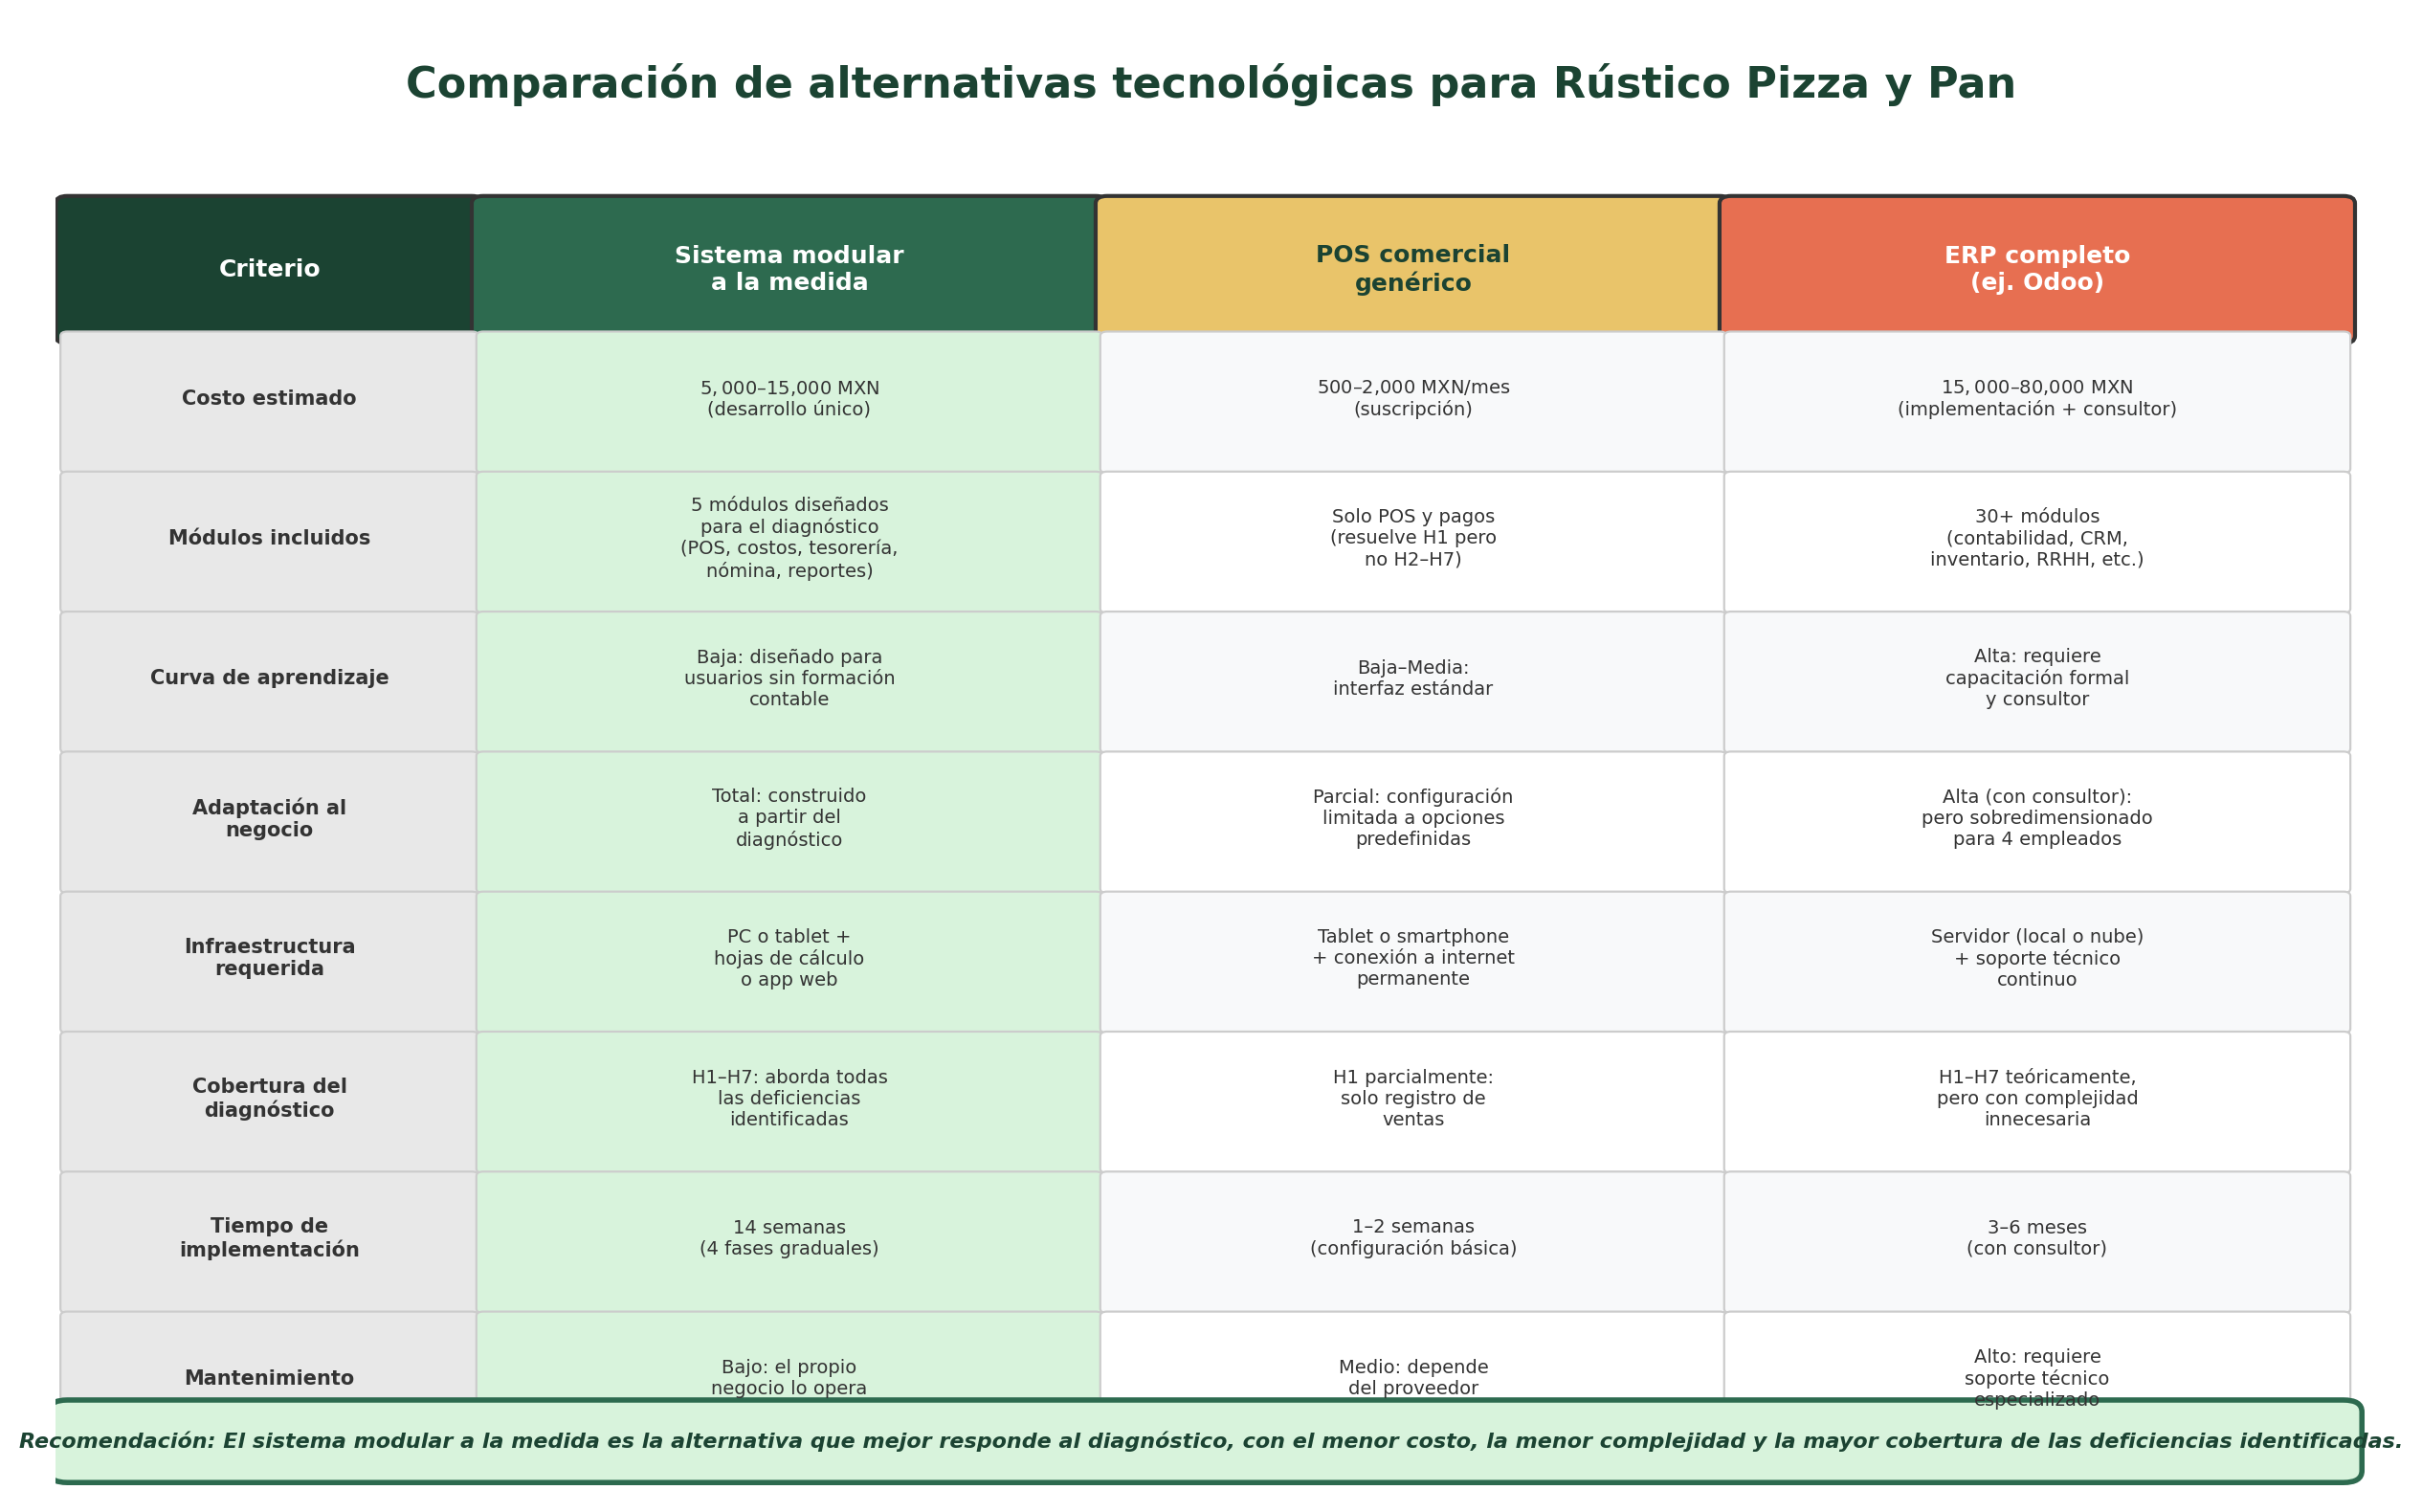
\includegraphics{diagramas/fig5_comparacion_soluciones.png}
\caption{Comparación de alternativas tecnológicas}
\end{figure}

\emph{Figura 5. Comparación de alternativas tecnológicas para Rústico
Pizza y Pan. El sistema modular a la medida ofrece la mayor cobertura de
las deficiencias diagnosticadas con el menor costo y la menor
complejidad.}

\hypertarget{arquitectura-del-sistema-propuesto}{%
\subsubsection{7.4.2 Arquitectura del sistema
propuesto}\label{arquitectura-del-sistema-propuesto}}

El sistema se estructura en cinco módulos interconectados que cubren el
ciclo financiero completo de una microempresa del sector restaurantero.
La arquitectura sigue un patrón de flujo descendente donde el Punto de
Venta actúa como generador primario de datos y el módulo de Reportes
como consumidor final.

\begin{figure}
\centering
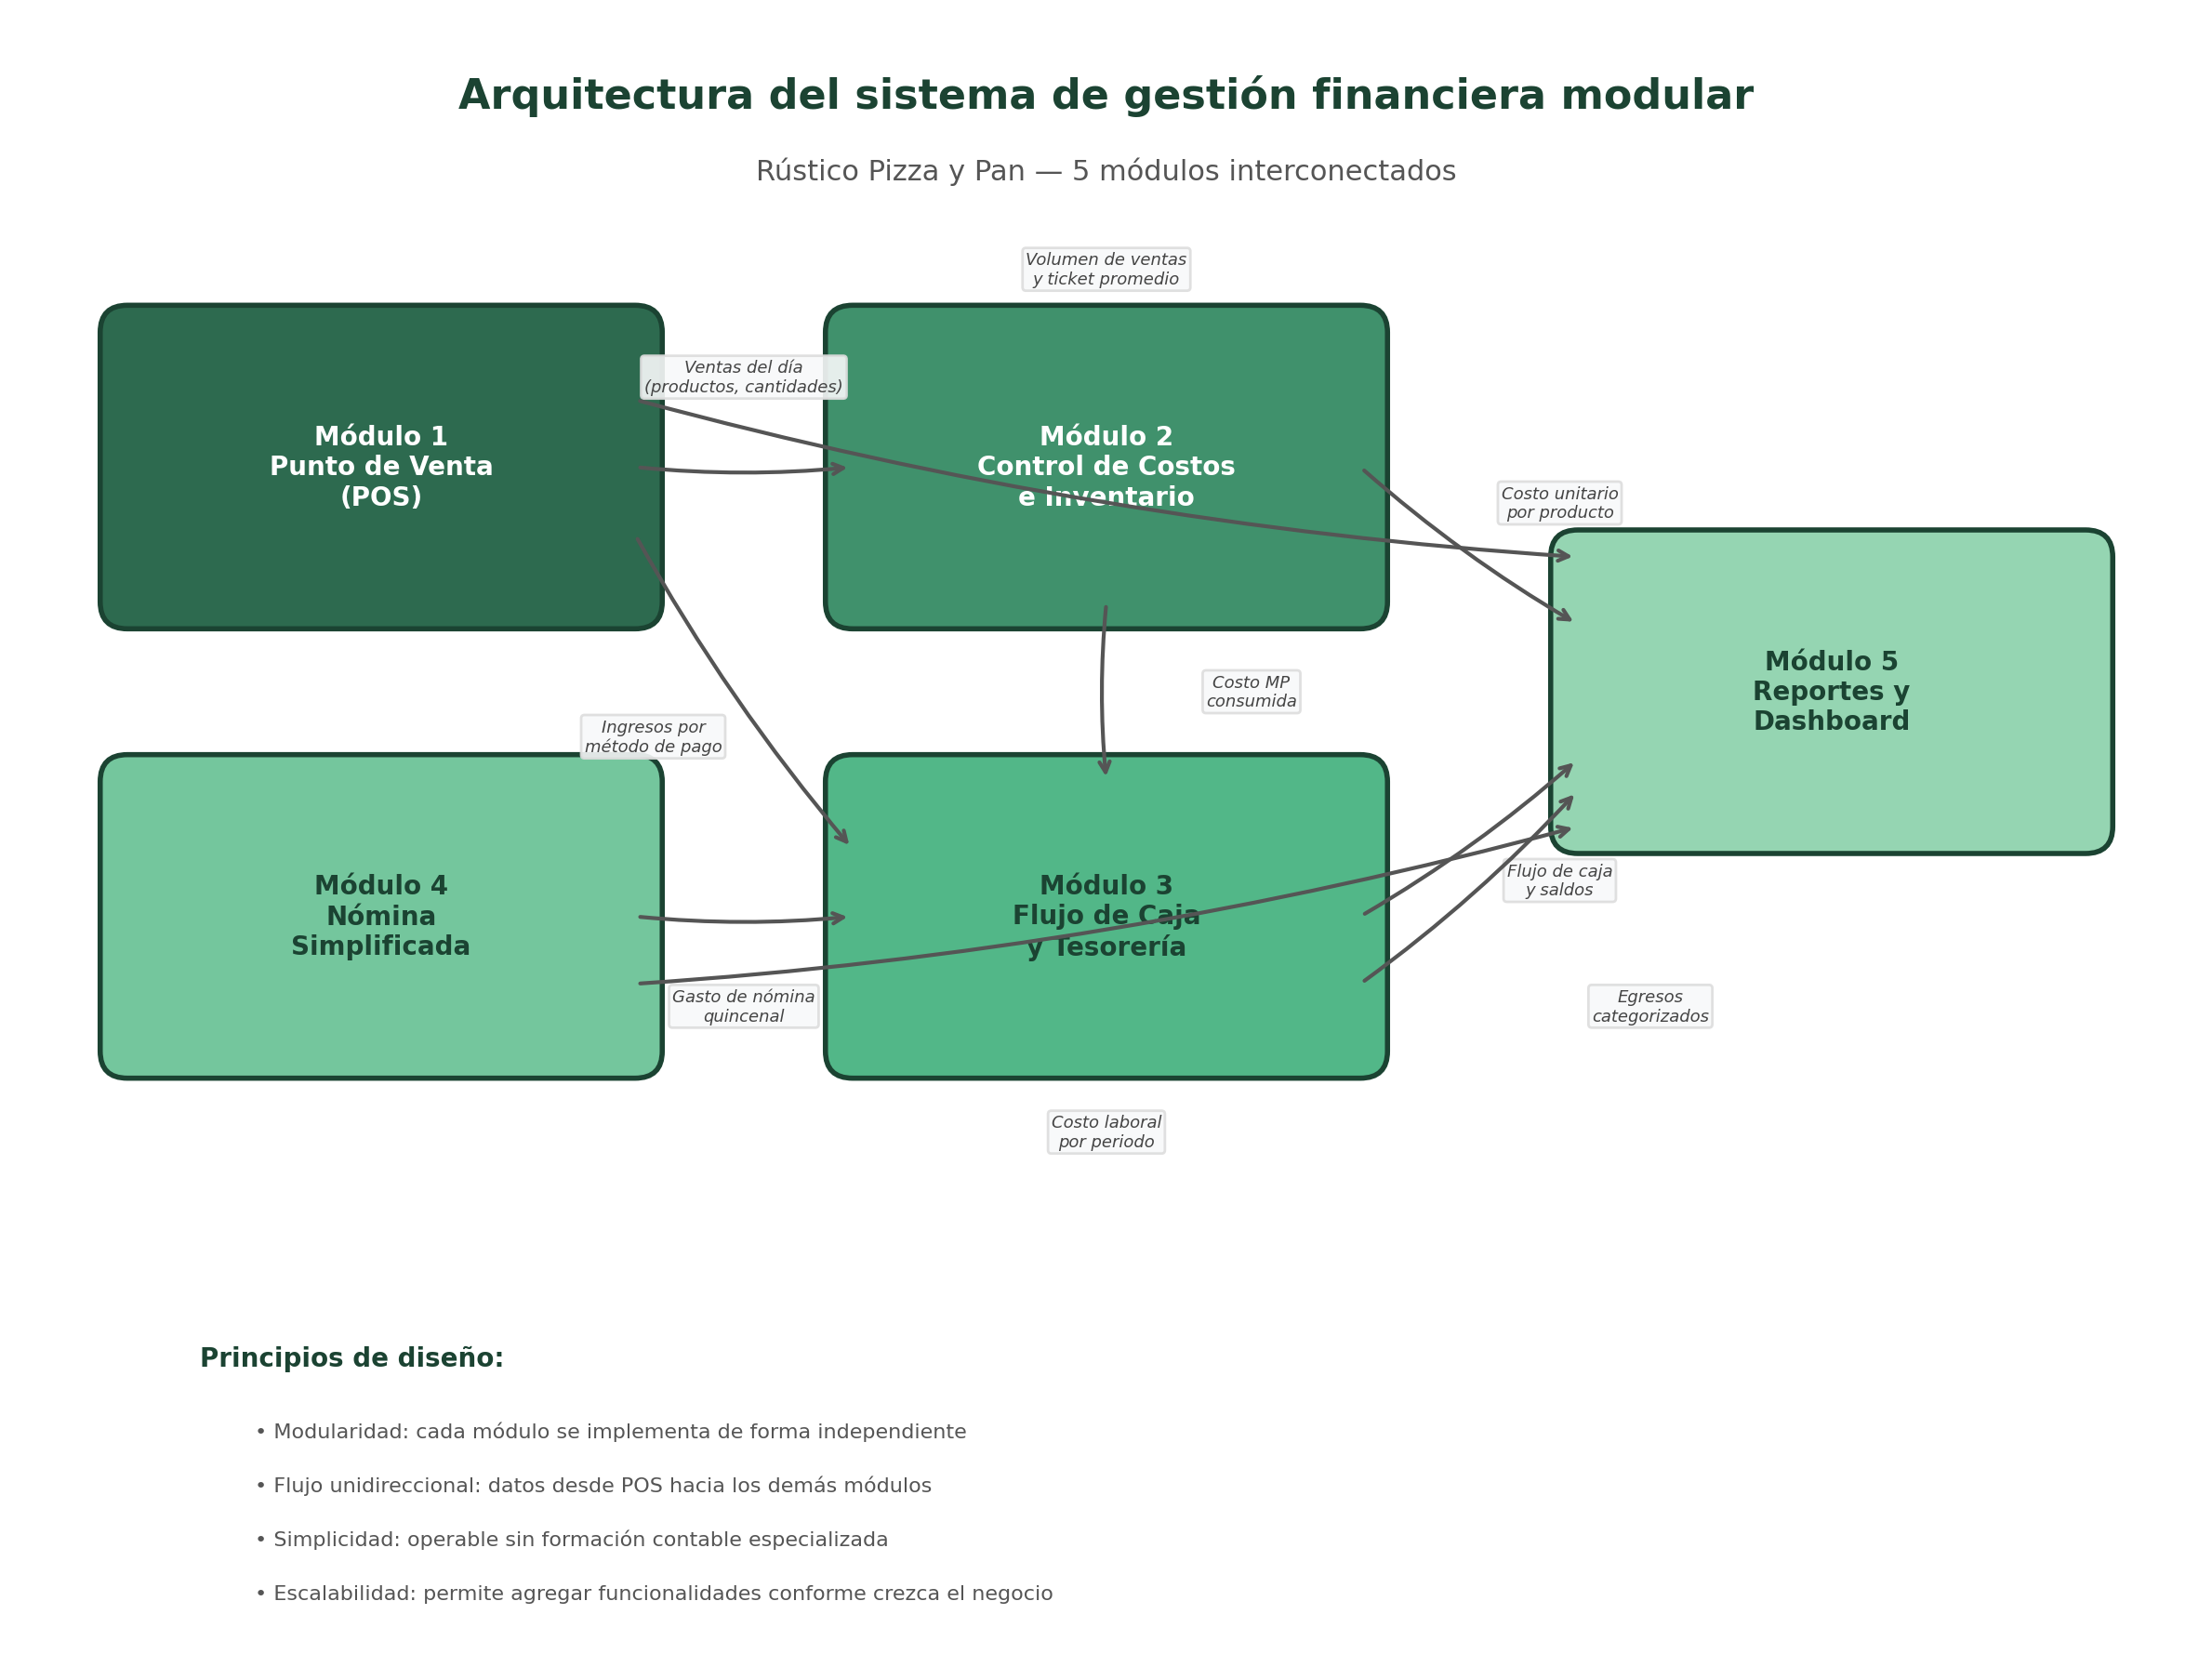
\includegraphics{diagramas/fig1_arquitectura_sistema.png}
\caption{Arquitectura del sistema de gestión financiera modular}
\end{figure}

\emph{Figura 1. Arquitectura del sistema de gestión financiera modular.
Los cinco módulos se interconectan siguiendo un flujo unidireccional de
datos desde el punto de venta hacia los reportes gerenciales.}

\textbf{Módulo 1 --- Punto de Venta (POS).} Su objetivo es registrar de
manera estructurada cada transacción de venta, capturando qué se vendió,
cuánto se cobró y cómo se pagó. Resuelve directamente el hallazgo H1
(registros de ventas incompletos): reemplaza el registro manual
incompleto por un flujo de datos estructurado que incluye el desglose
por producto, método de pago y hora. Genera el corte de caja diario de
manera automática, eliminando las discrepancias observadas en el 33.8\%
de los cortes revisados.

\textbf{Módulo 2 --- Control de Costos e Inventario.} Permite conocer el
costo real de elaboración de cada producto del menú mediante el registro
de recetas (BOM --- Bill of Materials) y el cálculo automático del costo
unitario. Resuelve los hallazgos H3 (ausencia de costeo formal) y H7
(falta de control de inventario). Cada venta registrada en el POS
descuenta automáticamente los insumos correspondientes del inventario y
genera alertas cuando un insumo cae por debajo del nivel mínimo, lo que
habría prevenido los dos episodios de desabasto documentados en el
periodo.

\textbf{Módulo 3 --- Flujo de Caja y Tesorería.} Registra todos los
ingresos y egresos del negocio de forma categorizada, concilia los
cobros con tarjeta contra los depósitos bancarios y separa formalmente
las finanzas personales de las del negocio. Resuelve los hallazgos H2
(gastos sin categorizar) y H4 (terminal sin conciliación). Implementa un
catálogo de cuentas simplificado que elimina la ambigüedad en la
nomenclatura de gastos.

\textbf{Módulo 4 --- Nómina Simplificada.} Formaliza el registro de los
pagos al personal, calcula el costo laboral real del negocio y genera
recibos que documentan cada pago. Resuelve el hallazgo H5 (nómina
informal). Con 4 empleados y pagos quincenales, no se requiere software
especializado; una plantilla estructurada es suficiente.

\textbf{Módulo 5 --- Reportes y Dashboard.} Consolida la información de
los cuatro módulos anteriores en indicadores clave de desempeño (KPIs) y
reportes visuales que permiten a Martín y Mariana tomar decisiones
informadas. Resuelve el hallazgo H6 (inexistencia de reportes).

Los principios de diseño del sistema son cuatro: \textbf{modularidad}
(cada módulo puede implementarse de forma independiente), \textbf{flujo
unidireccional de datos} (los datos se generan en el punto de venta y
fluyen sin duplicación), \textbf{simplicidad operativa} (diseñado para
usuarios sin formación contable) y \textbf{escalabilidad} (permite
incorporar funcionalidades adicionales conforme el negocio crezca).

\hypertarget{flujo-de-datos-del-sistema}{%
\subsubsection{7.4.3 Flujo de datos del
sistema}\label{flujo-de-datos-del-sistema}}

El siguiente diagrama representa el recorrido completo de los datos
desde que un cliente realiza un pedido hasta que la información se
consolida en los reportes gerenciales. Se ilustra cómo un solo evento
---una venta--- genera actualizaciones en múltiples módulos del sistema.

\begin{figure}
\centering
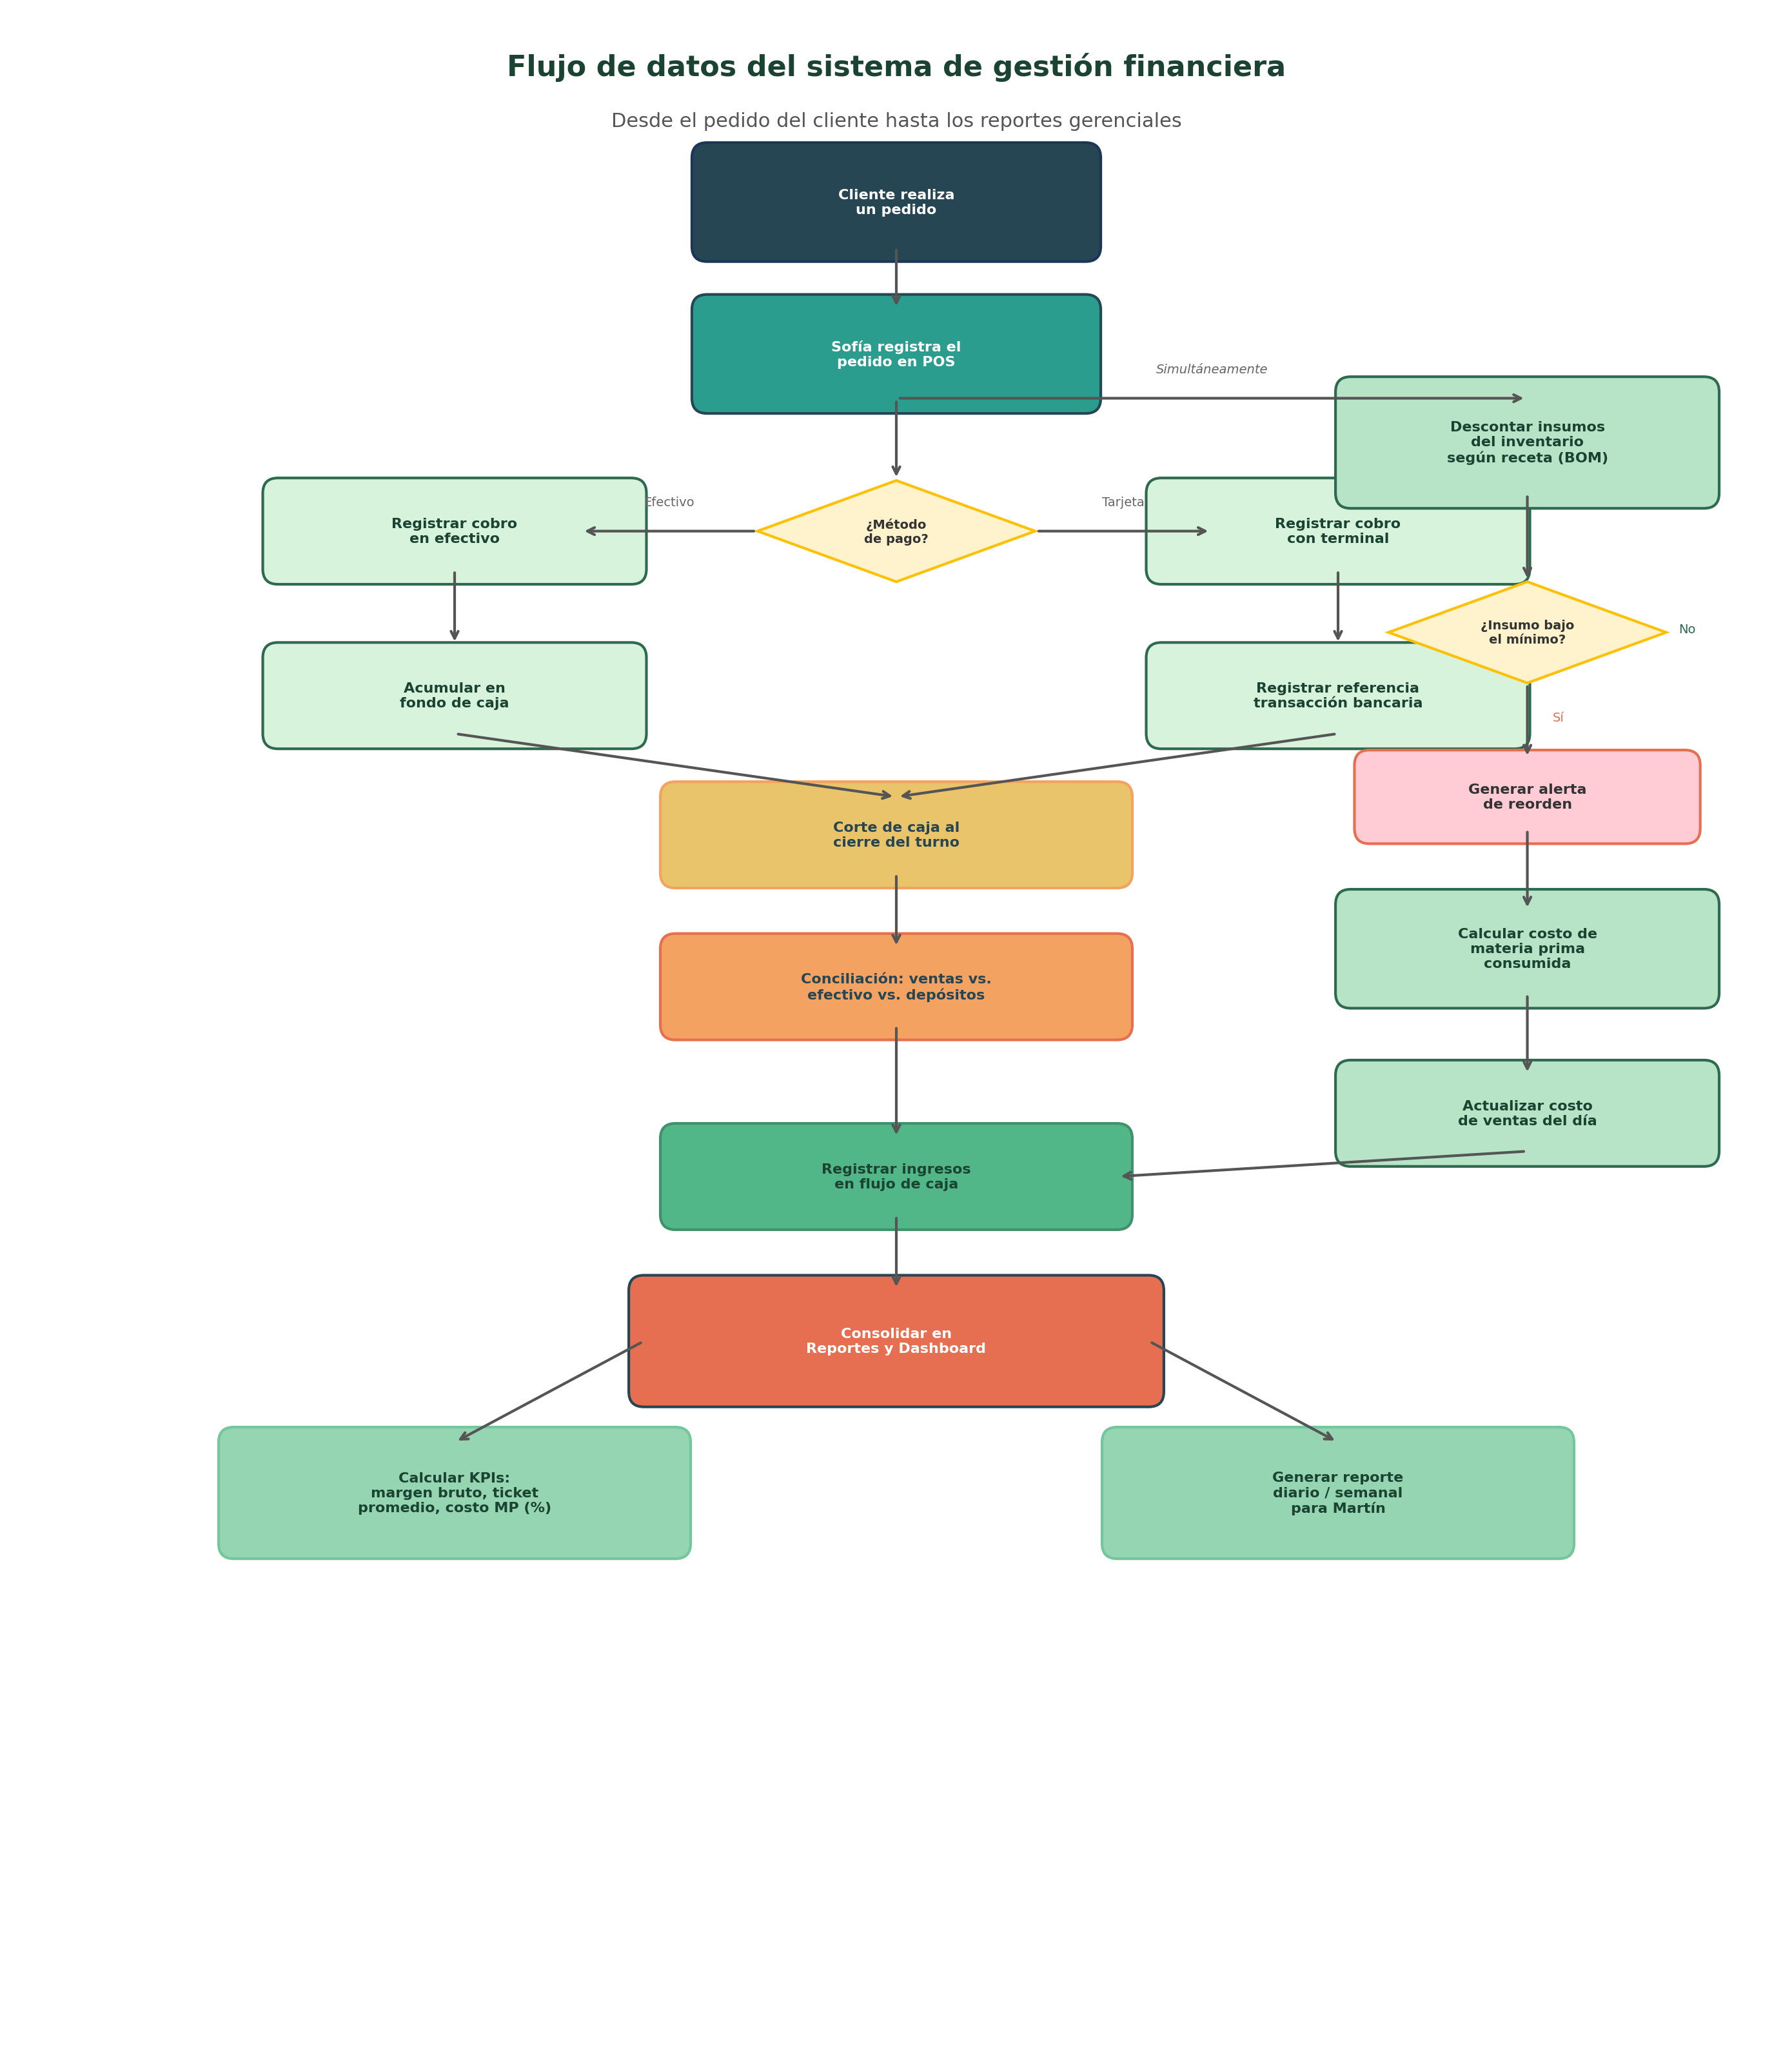
\includegraphics{diagramas/fig2_flujo_datos.png}
\caption{Flujo de datos del sistema de gestión financiera}
\end{figure}

\emph{Figura 2. Flujo de datos del sistema. Un solo evento (una venta)
genera actualizaciones simultáneas en los módulos de inventario,
tesorería y reportes.}

El flujo opera en seis pasos:

\begin{enumerate}
\def\labelenumi{\arabic{enumi}.}
\tightlist
\item
  \textbf{Origen.} El flujo inicia cuando un cliente realiza un pedido.
  Sofía, encargada de caja, registra el pedido en el módulo POS.
\item
  \textbf{Bifurcación por método de pago.} El sistema registra si el
  pago fue en efectivo o con tarjeta. Los pagos en efectivo se acumulan
  en el fondo de caja; los pagos con tarjeta generan una referencia
  bancaria para conciliación posterior.
\item
  \textbf{Impacto en inventario.} Simultáneamente, el sistema descuenta
  los insumos correspondientes del inventario según la receta (BOM) del
  producto vendido. Si algún insumo cae por debajo del nivel mínimo
  configurado, se genera una alerta de reorden.
\item
  \textbf{Cálculo de costo.} A partir de los insumos consumidos y sus
  costos unitarios registrados, el sistema calcula el costo de materia
  prima de cada venta y lo acumula en el costo de ventas del día.
\item
  \textbf{Conciliación.} Al cierre del turno, Sofía o Martín realizan el
  corte de caja. El sistema compara las ventas registradas con el
  efectivo contado y los vouchers de terminal, identificando
  discrepancias.
\item
  \textbf{Consolidación.} Todos los datos fluyen al módulo de Reportes,
  donde se calculan los KPIs y se generan los reportes periódicos para
  la toma de decisiones.
\end{enumerate}

\hypertarget{modelo-de-datos}{%
\subsubsection{7.4.4 Modelo de datos}\label{modelo-de-datos}}

El siguiente diagrama entidad-relación representa las principales
entidades de datos del sistema y sus relaciones. Se trata de un modelo
conceptual simplificado cuyo objetivo es ilustrar qué información
necesita capturar y relacionar el sistema.

\begin{figure}
\centering
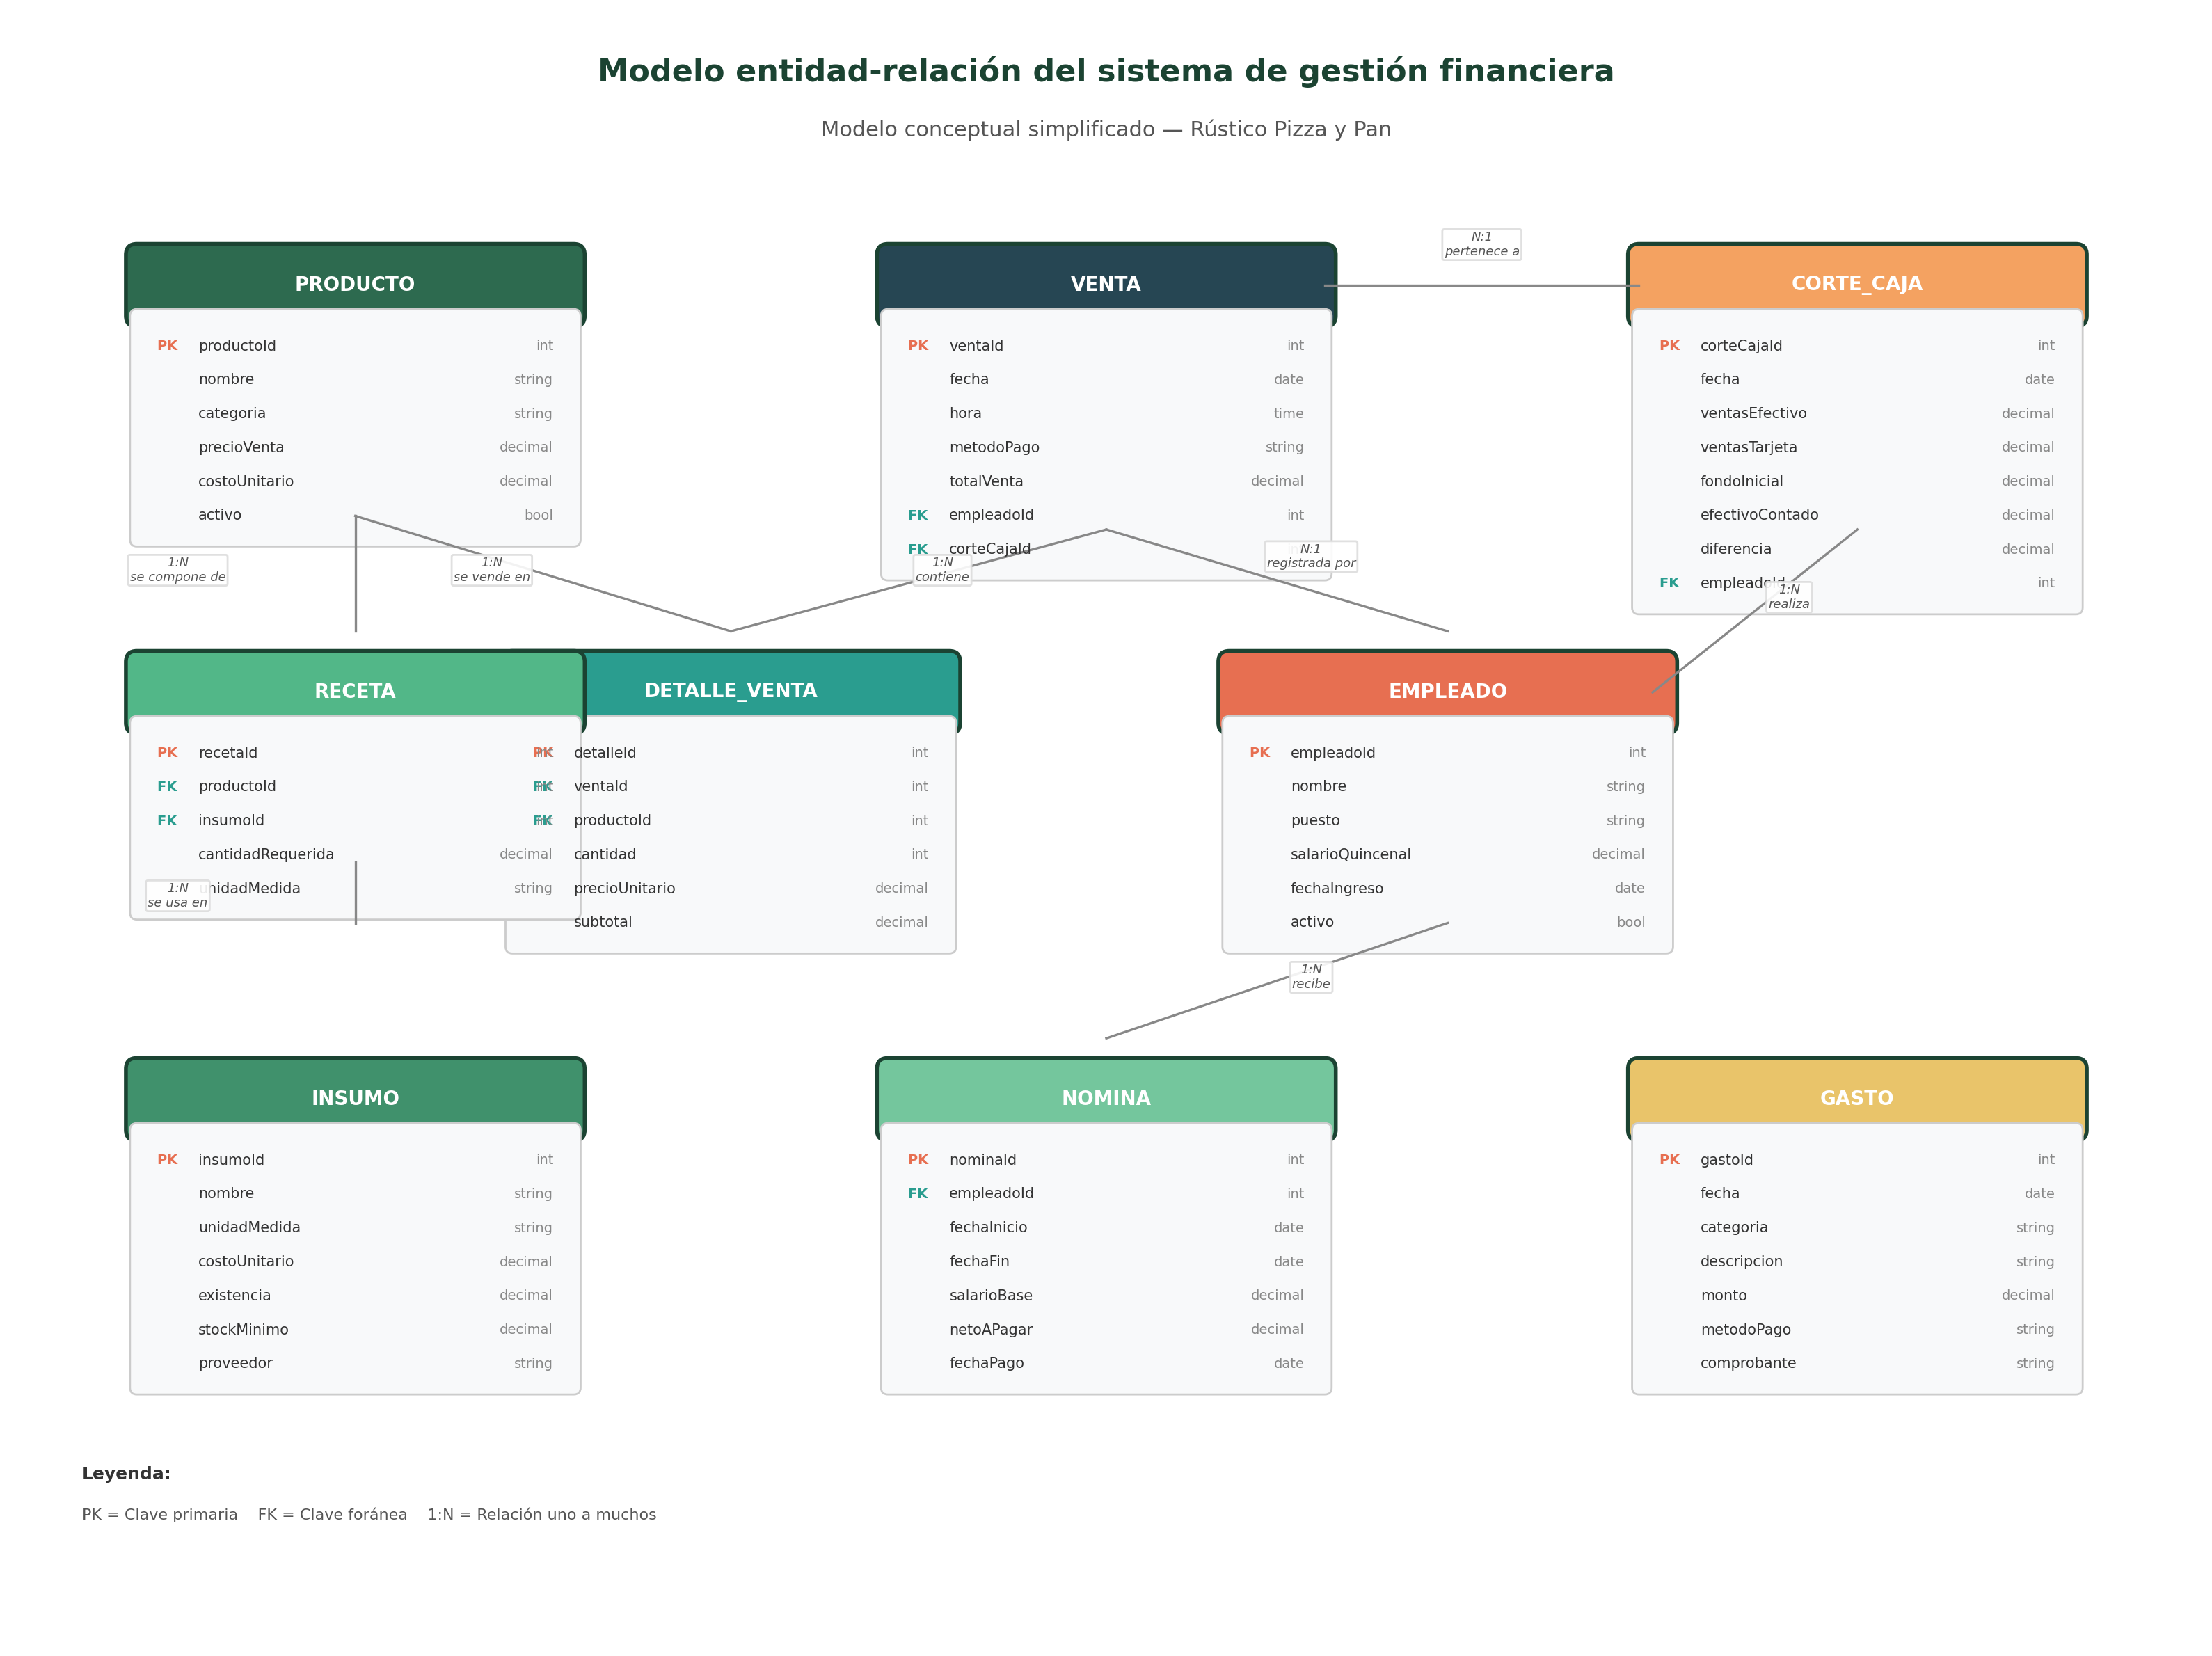
\includegraphics{diagramas/fig3_modelo_er.png}
\caption{Modelo entidad-relación del sistema}
\end{figure}

\emph{Figura 3. Modelo entidad-relación simplificado. Las nueve
entidades del sistema (Producto, Venta, DetalleVenta, Insumo, Receta,
Gasto, CorteCaja, Empleado, Nómina) representan las unidades de
información necesarias para integrar la gestión financiera del negocio.}

El modelo contempla nueve entidades principales:

\begin{longtable}[]{@{}lll@{}}
\toprule
\begin{minipage}[b]{0.30\columnwidth}\raggedright
Entidad\strut
\end{minipage} & \begin{minipage}[b]{0.30\columnwidth}\raggedright
Descripción\strut
\end{minipage} & \begin{minipage}[b]{0.30\columnwidth}\raggedright
Registros estimados\strut
\end{minipage}\tabularnewline
\midrule
\endhead
\begin{minipage}[t]{0.30\columnwidth}\raggedright
\textbf{Producto}\strut
\end{minipage} & \begin{minipage}[t]{0.30\columnwidth}\raggedright
Cada artículo del menú: pizzas, panes, postres, bebidas. Incluye precio
de venta y costo unitario calculado a partir de la receta\strut
\end{minipage} & \begin{minipage}[t]{0.30\columnwidth}\raggedright
\textasciitilde30 a 40 productos activos\strut
\end{minipage}\tabularnewline
\begin{minipage}[t]{0.30\columnwidth}\raggedright
\textbf{Venta}\strut
\end{minipage} & \begin{minipage}[t]{0.30\columnwidth}\raggedright
Cada transacción individual con un cliente. Registra fecha, hora, método
de pago y el empleado que la registró\strut
\end{minipage} & \begin{minipage}[t]{0.30\columnwidth}\raggedright
\textasciitilde30 a 60 ventas diarias\strut
\end{minipage}\tabularnewline
\begin{minipage}[t]{0.30\columnwidth}\raggedright
\textbf{DetalleVenta}\strut
\end{minipage} & \begin{minipage}[t]{0.30\columnwidth}\raggedright
Líneas individuales de cada venta (qué producto, cuántas unidades, a qué
precio)\strut
\end{minipage} & \begin{minipage}[t]{0.30\columnwidth}\raggedright
\textasciitilde50 a 100 líneas diarias\strut
\end{minipage}\tabularnewline
\begin{minipage}[t]{0.30\columnwidth}\raggedright
\textbf{Insumo}\strut
\end{minipage} & \begin{minipage}[t]{0.30\columnwidth}\raggedright
Cada materia prima: harina, queso mozzarella, pepperoni, tomate,
levadura, etc.\strut
\end{minipage} & \begin{minipage}[t]{0.30\columnwidth}\raggedright
\textasciitilde50 a 80 insumos\strut
\end{minipage}\tabularnewline
\begin{minipage}[t]{0.30\columnwidth}\raggedright
\textbf{Receta (BOM)}\strut
\end{minipage} & \begin{minipage}[t]{0.30\columnwidth}\raggedright
Lista de materiales por producto: qué insumos y en qué cantidad se
necesitan para una unidad\strut
\end{minipage} & \begin{minipage}[t]{0.30\columnwidth}\raggedright
\textasciitilde150 a 250 relaciones\strut
\end{minipage}\tabularnewline
\begin{minipage}[t]{0.30\columnwidth}\raggedright
\textbf{Gasto}\strut
\end{minipage} & \begin{minipage}[t]{0.30\columnwidth}\raggedright
Cada erogación que no sea compra de insumos: renta, gas, luz,
mantenimiento, publicidad\strut
\end{minipage} & \begin{minipage}[t]{0.30\columnwidth}\raggedright
\textasciitilde30 a 50 gastos mensuales\strut
\end{minipage}\tabularnewline
\begin{minipage}[t]{0.30\columnwidth}\raggedright
\textbf{CorteCaja}\strut
\end{minipage} & \begin{minipage}[t]{0.30\columnwidth}\raggedright
Registro del cierre diario de caja: ventas, efectivo contado, tarjeta,
diferencia\strut
\end{minipage} & \begin{minipage}[t]{0.30\columnwidth}\raggedright
1 por día operativo (\textasciitilde26/mes)\strut
\end{minipage}\tabularnewline
\begin{minipage}[t]{0.30\columnwidth}\raggedright
\textbf{Empleado}\strut
\end{minipage} & \begin{minipage}[t]{0.30\columnwidth}\raggedright
Datos de cada miembro del equipo: Martín, Mariana, Luis Ángel,
Sofía\strut
\end{minipage} & \begin{minipage}[t]{0.30\columnwidth}\raggedright
4 registros activos\strut
\end{minipage}\tabularnewline
\begin{minipage}[t]{0.30\columnwidth}\raggedright
\textbf{Nómina}\strut
\end{minipage} & \begin{minipage}[t]{0.30\columnwidth}\raggedright
Registro de cada pago: salario base, deducciones, neto pagado, fecha y
método\strut
\end{minipage} & \begin{minipage}[t]{0.30\columnwidth}\raggedright
\textasciitilde8 registros mensuales\strut
\end{minipage}\tabularnewline
\bottomrule
\end{longtable}

La pieza clave del modelo es la entidad \textbf{Receta}, que vincula
cada producto del menú con los insumos que lo componen. Esta relación es
la que permite que una venta registrada en el POS genere automáticamente
el descuento de inventario y el cálculo de costo de materia prima,
resolviendo la desconexión entre ventas y costos que el diagnóstico
identificó como una de las brechas más críticas.

\hypertarget{implementaciuxf3n-por-fases-y-kpis}{%
\subsubsection{7.4.5 Implementación por fases y
KPIs}\label{implementaciuxf3n-por-fases-y-kpis}}

Dada la naturaleza del negocio ---microempresa con 4 empleados, sin
personal de TI, sin experiencia previa en sistemas de gestión---, se
propone una implementación gradual en cuatro fases que minimice la
disrupción operativa y permita la adopción progresiva.

\begin{longtable}[]{@{}clcl@{}}
\toprule
\begin{minipage}[b]{0.28\columnwidth}\centering
Fase\strut
\end{minipage} & \begin{minipage}[b]{0.17\columnwidth}\raggedright
Módulos\strut
\end{minipage} & \begin{minipage}[b]{0.28\columnwidth}\centering
Duración estimada\strut
\end{minipage} & \begin{minipage}[b]{0.17\columnwidth}\raggedright
Objetivo\strut
\end{minipage}\tabularnewline
\midrule
\endhead
\begin{minipage}[t]{0.28\columnwidth}\centering
\textbf{1}\strut
\end{minipage} & \begin{minipage}[t]{0.17\columnwidth}\raggedright
Punto de Venta (POS) + Corte de Caja\strut
\end{minipage} & \begin{minipage}[t]{0.28\columnwidth}\centering
4 semanas\strut
\end{minipage} & \begin{minipage}[t]{0.17\columnwidth}\raggedright
Capturar el dato de origen: cada venta con desglose de producto y método
de pago. Establecer la disciplina del corte de caja diario\strut
\end{minipage}\tabularnewline
\begin{minipage}[t]{0.28\columnwidth}\centering
\textbf{2}\strut
\end{minipage} & \begin{minipage}[t]{0.17\columnwidth}\raggedright
Flujo de Caja y Tesorería\strut
\end{minipage} & \begin{minipage}[t]{0.28\columnwidth}\centering
3 semanas\strut
\end{minipage} & \begin{minipage}[t]{0.17\columnwidth}\raggedright
Categorizar egresos, separar finanzas personales del negocio, iniciar la
conciliación bancaria\strut
\end{minipage}\tabularnewline
\begin{minipage}[t]{0.28\columnwidth}\centering
\textbf{3}\strut
\end{minipage} & \begin{minipage}[t]{0.17\columnwidth}\raggedright
Control de Costos e Inventario\strut
\end{minipage} & \begin{minipage}[t]{0.28\columnwidth}\centering
4 semanas\strut
\end{minipage} & \begin{minipage}[t]{0.17\columnwidth}\raggedright
Registrar recetas (BOM), calcular costos unitarios, establecer control
de existencias de los 15-20 insumos principales\strut
\end{minipage}\tabularnewline
\begin{minipage}[t]{0.28\columnwidth}\centering
\textbf{4}\strut
\end{minipage} & \begin{minipage}[t]{0.17\columnwidth}\raggedright
Nómina Simplificada + Reportes y Dashboard\strut
\end{minipage} & \begin{minipage}[t]{0.28\columnwidth}\centering
3 semanas\strut
\end{minipage} & \begin{minipage}[t]{0.17\columnwidth}\raggedright
Formalizar los pagos al personal, activar los KPIs y los reportes
consolidados\strut
\end{minipage}\tabularnewline
\bottomrule
\end{longtable}

\textbf{Duración total estimada:} 14 semanas (aproximadamente 3.5
meses).

Los indicadores clave de desempeño (KPIs) propuestos están diseñados
para ser comprensibles para un propietario sin formación contable,
calculables con los datos que genera el sistema y accionables en el
corto plazo:

\begin{longtable}[]{@{}llcc@{}}
\toprule
\begin{minipage}[b]{0.17\columnwidth}\raggedright
KPI\strut
\end{minipage} & \begin{minipage}[b]{0.17\columnwidth}\raggedright
Fórmula\strut
\end{minipage} & \begin{minipage}[b]{0.28\columnwidth}\centering
Frecuencia\strut
\end{minipage} & \begin{minipage}[b]{0.28\columnwidth}\centering
Meta\strut
\end{minipage}\tabularnewline
\midrule
\endhead
\begin{minipage}[t]{0.17\columnwidth}\raggedright
\textbf{Margen bruto (\%)}\strut
\end{minipage} & \begin{minipage}[t]{0.17\columnwidth}\raggedright
(Ventas − Costo MP) ÷ Ventas × 100\strut
\end{minipage} & \begin{minipage}[t]{0.28\columnwidth}\centering
Diaria / Semanal\strut
\end{minipage} & \begin{minipage}[t]{0.28\columnwidth}\centering
≥ 65\%\strut
\end{minipage}\tabularnewline
\begin{minipage}[t]{0.17\columnwidth}\raggedright
\textbf{Ticket promedio (\$)}\strut
\end{minipage} & \begin{minipage}[t]{0.17\columnwidth}\raggedright
Ventas totales ÷ Número de transacciones\strut
\end{minipage} & \begin{minipage}[t]{0.28\columnwidth}\centering
Diaria\strut
\end{minipage} & \begin{minipage}[t]{0.28\columnwidth}\centering
\$250 --
\(400 MXN | | **Costo de materia prima (%)** | Costo MP consumida ÷ Ventas totales × 100 | Semanal | ≤ 30 – 35% | | **Rotación de inventario** | Costo MP consumida ÷ Inventario promedio | Mensual | 8 – 12 veces/mes | | **Punto de equilibrio (
\))**\strut
\end{minipage}\tabularnewline
\begin{minipage}[t]{0.17\columnwidth}\raggedright
\textbf{Diferencia en corte de caja (\%)}\strut
\end{minipage} & \begin{minipage}[t]{0.17\columnwidth}\raggedright
(Efectivo contado − Efectivo esperado) ÷ Efectivo esperado × 100\strut
\end{minipage} & \begin{minipage}[t]{0.28\columnwidth}\centering
Diaria\strut
\end{minipage} & \begin{minipage}[t]{0.28\columnwidth}\centering
≤ ±1\%\strut
\end{minipage}\tabularnewline
\begin{minipage}[t]{0.17\columnwidth}\raggedright
\textbf{Productividad por empleado}\strut
\end{minipage} & \begin{minipage}[t]{0.17\columnwidth}\raggedright
Ventas totales ÷ Número de empleados\strut
\end{minipage} & \begin{minipage}[t]{0.28\columnwidth}\centering
Mensual\strut
\end{minipage} & \begin{minipage}[t]{0.28\columnwidth}\centering
≥ \$20,000 MXN/empleado\strut
\end{minipage}\tabularnewline
\begin{minipage}[t]{0.17\columnwidth}\raggedright
\textbf{Días con registro completo (\%)}\strut
\end{minipage} & \begin{minipage}[t]{0.17\columnwidth}\raggedright
Días con registro ÷ Días operativos × 100\strut
\end{minipage} & \begin{minipage}[t]{0.28\columnwidth}\centering
Mensual\strut
\end{minipage} & \begin{minipage}[t]{0.28\columnwidth}\centering
100\%\strut
\end{minipage}\tabularnewline
\bottomrule
\end{longtable}

\hypertarget{impacto-esperado-en-el-corto-y-largo-plazo}{%
\subsubsection{7.4.6 Impacto esperado en el corto y largo
plazo}\label{impacto-esperado-en-el-corto-y-largo-plazo}}

\textbf{Impacto en el corto plazo (primer año).}

La sistematización del registro de ventas mediante el módulo POS
eliminará los días sin registro y permitirá el desglose por producto,
método de pago y hora. La meta es llevar el porcentaje de días con
registro completo del 89.7\% actual al 100\%. Simultáneamente, la
digitalización de la libreta de gastos con catálogo de cuentas
predefinido reducirá el subregistro del 87.4\% actual al 98\% en los
primeros seis meses.

La actualización de la tabla de costos por producto, incorporando los
precios vigentes de insumos y los costos indirectos de producción,
permitirá conocer el margen bruto real de cada producto. Se espera que
esta actualización revele que los márgenes reales son entre 3 y 7 puntos
porcentuales inferiores a los percibidos actualmente, lo que
fundamentará decisiones de ajuste de precios o reformulación de recetas.

La separación de cuentas bancarias y la implementación de conciliaciones
semanales eliminarán las distorsiones causadas por la mezcla de fondos.
La meta es reducir el porcentaje de cortes con diferencias del 33.8\%
actual a menos del 5\%.

La implementación de un sistema de inventario con niveles mínimos de
reorden para los 15-20 insumos principales reducirá los episodios de
desabasto y permitirá cuantificar la merma real.

En su conjunto, el impacto en el corto plazo se valora como
\textbf{favorable}: las mejoras propuestas atienden directamente las
brechas documentadas y cada una cuenta con un indicador medible. Medina
y Aguilar (2013) han documentado que la calidad de la información
financiera en los sistemas contables de las pequeñas empresas tiene una
influencia positiva y significativa en la toma de decisiones
gerenciales, lo que es consistente con los resultados esperados de este
diagnóstico.\footnote{Medina, J. y Aguilar, P. (2013). Sistemas de
  información financiera y su impacto en las PYMES. \emph{Acta
  Universitaria}, 23(1), 49-57. https://doi.org/10.15174/au.2013.515}

\textbf{Impacto en el largo plazo (más de un año).}

\emph{Planeación estratégica.} Con un mínimo de 12 meses de datos
financieros completos y confiables, Rústico podrá generar por primera
vez estados de resultados mensuales formales que reflejen con precisión
los ingresos, costos y gastos del negocio. Esto permitirá calcular la
utilidad neta real (actualmente desconocida) y establecer metas de
crecimiento fundamentadas. El conocimiento del punto de equilibrio
---estimado preliminarmente en \$75,200 mensuales con base en costos
fijos de \$37,600 y un margen de contribución del 50\%--- proporcionará
un referente cuantitativo para evaluar el desempeño.

\emph{Formalización y cumplimiento fiscal.} Actualmente, el negocio está
inscrito en el RESICO y emite únicamente 3 a 4 facturas mensuales. La
información financiera ordenada facilitará el cumplimiento fiscal
progresivo y, a largo plazo, habilitará el acceso a instrumentos que
requieren documentación formal: líneas de crédito bancario, programas de
apoyo gubernamental para microempresas y financiamiento para inversión
en equipo o expansión. La meta es incrementar el porcentaje de ingresos
documentados fiscalmente del estimado actual (menos del 5\%) al 50\% en
un plazo de 18 a 24 meses.

\emph{Competitividad y permanencia.} La gestión financiera basada en
datos permitirá a Rústico tomar decisiones más acertadas sobre precios,
composición del menú, horarios de operación, negociación con proveedores
y evaluación de nuevos canales de venta. García-Moreno et al.~(2019)
sostienen que la gestión financiera integral ``genera oportunidades para
la creación de ventajas competitivas sostenidas y la adaptación a los
cambios del entorno empresarial, siendo la información contable un
recurso estratégico para el manejo, control y la competitividad de la
empresa''.\footnote{García-Moreno, S. M., Montoya-del-Corte, J. y
  Fernández-Laviada, A. (2019). Financial management practices in small
  enterprises: an empirical study. \emph{International Journal of
  Entrepreneurial Behaviour and Research}, 25(8), 1751-1776.
  https://doi.org/10.1108/IJEBR-11-2018-0726}

En su conjunto, el impacto a largo plazo se valora como
\textbf{favorable}: la información financiera confiable no solo mejora
la gestión operativa inmediata, sino que habilita el crecimiento
estratégico, la formalización gradual y la resiliencia ante condiciones
adversas del entorno, factores que determinan la permanencia de las
microempresas en el mercado mexicano.

\begin{center}\rule{0.5\linewidth}{0.5pt}\end{center}

\end{document}
